\documentclass[12pt]{article}

\usepackage{notestyle}

\graphicspath{{./img/}}


\title{Appunti Reti2}
\author{Brendon Mendicino}



\begin{document}

\maketitle
\newpage
\tableofcontents
\newpage


\section{Introduzione}\label{sec:introduzione}
...


\section{Multicast}
Gli indirizzi che identificano dei gruppi multicast sono quelli di tipo D, iniziano con 1110 ($224.0.0.0 - 239.255.255.255$).

Si prendono i 23 bit bassi dell'IP e vengono assegnati ai 23 bit bassi dell'indirizzo MAC multicast, questa operazione si chiama di \textbf{join} ad un gruppo multicast. Questo approccio potrebbe portare a dei conflitti, la probalit\`a che una collisione avvenga \`e molto bassa ma non \`e zero, i conflitti comportano ricevere il traffico di un altro gruppo multicast anche se non abbiamo fatto un join con quello.

Esempio: viene usato l'indirizzo 224.0.0.0 come un gruppo multicast, gli host che vogliono connettersi a questo gruppo dovranno fare il join, e quindi impostare la loro scheda di rete (solitamente una scheda di rete virtuale, in cui viene aggiunto il MAC multicast) con il MAC multicast, in questo caso gli ultimi 23 bit saranno a 0.


\newpage
\section{IPv6}
Gli indirizzi ipv6 sono rappresentati su 128, quindi si hanno $2^{128}$ combinazioni. Per rappresentarli si divide l'indirizzo in 8 gruppi di 2 byte, separati da un ":". Ci sono delle strategie per rendere pi\`u leggibile l'indirizzo:
\begin{enumerate}
    \item gli zeri in fronte possono essere omessi;
    \item gli zeri (":0:") posso essere sostituiti con un "::" solo una volta;
\end{enumerate}

Per rappresentare l'indirizzo di rete si usano 64 bit. Il concetto di aggregazione gerarchico viene mentenuto del prefix length e dalla netmask, dunque il prefix viene usato per il subnetting.

I principi di assegnamento sono:
\begin{itemize}
    \item \textbf{subnetwork}: set of host with the same prefix;
    \item \textbf{link}: physical network;
    \item \textbf{on-link}: comunicazioni tra host con lo stesso prefisso;
    \item \textbf{off-link}: comunicazioni tra host con prefisso diverso;
\end{itemize}

\subsection{Tipologie di Indirizzi}
\begin{figure}[H]
    \centering
    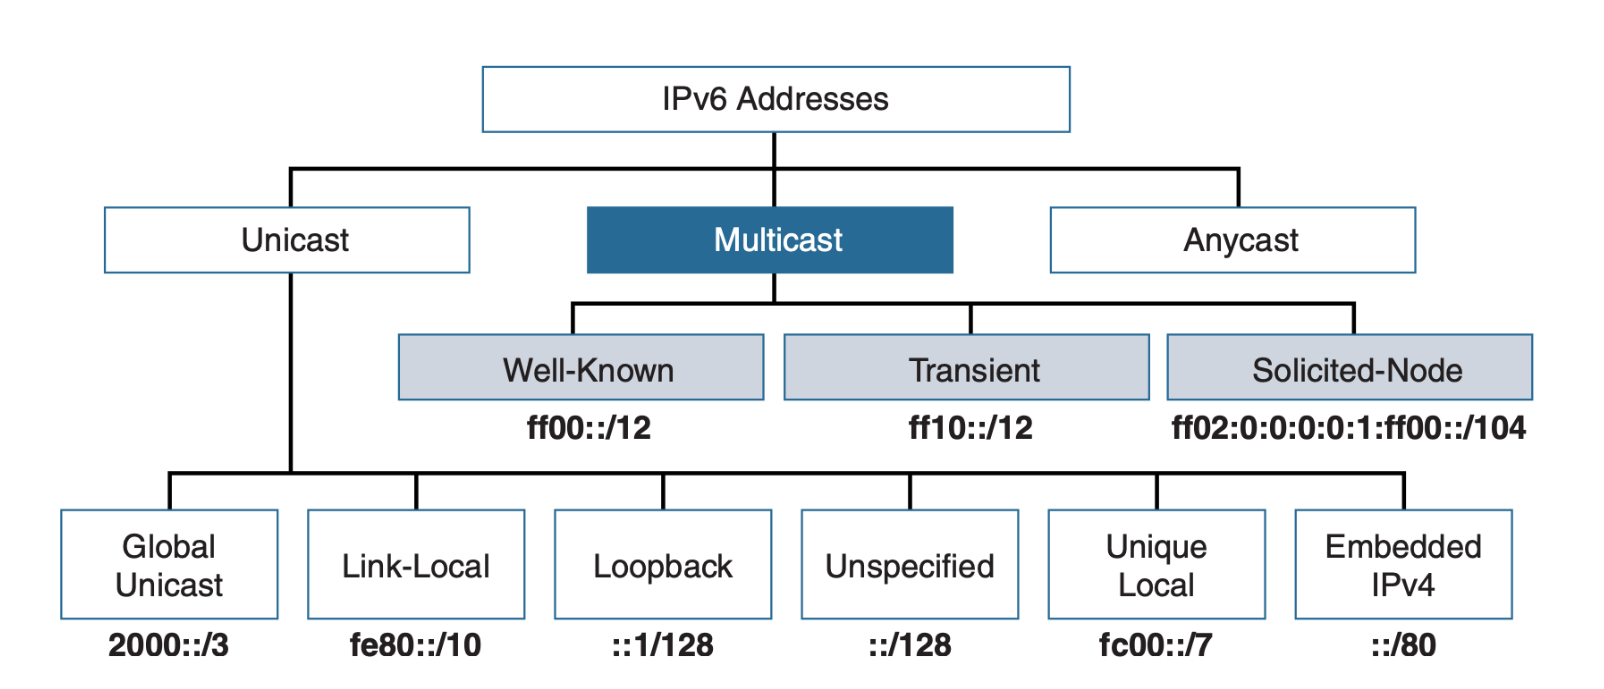
\includegraphics[width=1\textwidth]{ipv6-spazio-di-indirizzamento.png}
    \caption{Ipv6 Spazio Di Indirizzamento}
    \label{fig:ipv6-spazio-di-indirizzamento}
\end{figure}
\subsubsection{Indirizzi Multicast}
\tolerance=1000
Il multicast ha una rappresentazione simile ad IPv4, infatti hanno un range di FF00::/8 (1111 1111 ...), che si dividono in tre sottocategorie:
\begin{itemize}
    \item \textbf{well-known multicast} FF00::/12 (1111 1111 0000 ...) : questo range di indirizzi \`e assegnato dalla IANA, utilizzato dalgi ISP per scopi di comunicazione;
    \item \textbf{transient} FF10::/12 (1111 1111 0001 ...): assegnati dinamicamente;
    \item \textbf{solicited-node multicast} FF02:0:0:0:0:1:FF00::/104: simile al broadcast address in ARP;
\end{itemize}
Un indirizzo multicast \`e formato da:
\begin{itemize}
    \tolerance=1000
    \item I primi 8 bit mi identificano un indirizzo multicast, tutti settati ad 1;
    \item 4 bit assegnati a dei flag: l'unico utilizzabile \`e il campo T che specifica se l'indirizzo \`e permanente (0), ovvero assegnato dalla IANA, oppure non-permanente (1), gli altri campi non hanno un'assegnazione;
    \item 4 bit per stabilire lo \textbf{scope}, definisce il range di indirizzi multicast;
    \item gli ultimi 112 rappresentano il \textbf{group id};    
\end{itemize}
\begin{figure}[H]
    \centering
    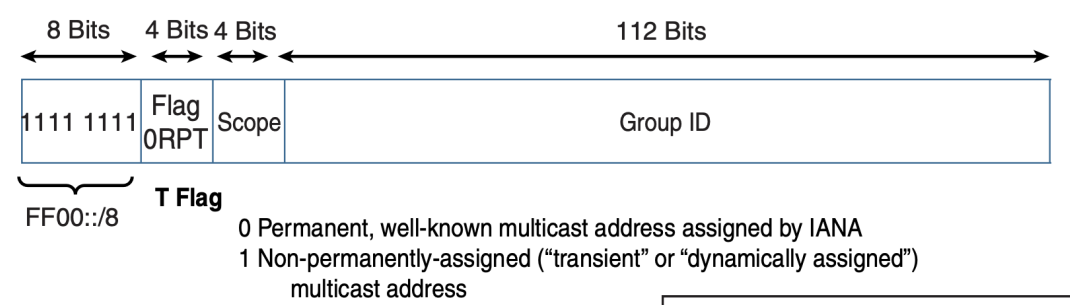
\includegraphics[width=0.8\textwidth]{indirizzo-multicast.png}
    \caption{Indirizzo Multicast}
    \label{fig:indirizzo-multicast}
\end{figure}



\subsubsection{Indirizzi Global Unicast}
Sono l'equivalte degli indirizzi publici IPv4. Quando un nuovo host si collega alla rete, sa automaticamente il suo indirizzo, infatti gli indirizzi unicast sono plug and play. Gli indirizzi sono composti da tutto la spazio 2000::/3, l'indirizzo si divede in:
\begin{itemize}
    \item 3 bit: 001;
    \item n bit: global routing prefix;
    \item m bit: subnet ID;
    \item $128-m-n-3$ bit: interface ID;
\end{itemize}
Il prefisso moderno \`e stato assegnato formalmente da entit\`a multi-livello:
\begin{itemize}
    \item 3 bit: 001;
    \item 13 bit: TLA ID, Top Level Authority (Large ISP);
    \item 32 bit: NLA ID, Next Level Authority (Organizzazione);
    \item 16 bit: SLA ID, Subnet Level Authority;
    \item 64 bit: Interface ID;
\end{itemize}
\begin{figure}[H]
    \centering
    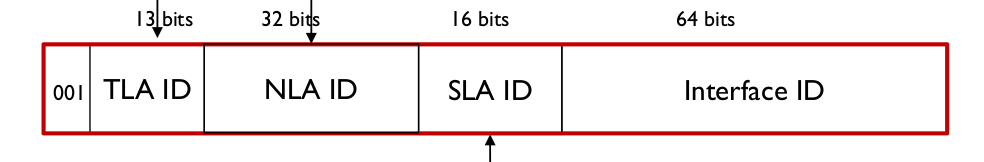
\includegraphics[width=1\textwidth]{indirizzo-global-unicast.png}
    \caption{Indirizzo Global Unicast}
    \label{fig:indirizzo-global-unicast}
\end{figure}


\subsubsection{Link Local/Site Local}
Gli indirizzi link/site local sono assegnati automaticamente, fanno parte del gruppo fe80::/9 (1111 1110 1...), e si distinguono in:
\begin{itemize}
    \item \textbf{link-local} fe80::/10 (1111 1110 10...): vengono generati automaticamente, ogni host in una rete ipv6 deve avare un link-local address utilizzato per comunicazioni di \textbf{neighbor discovery};
    \item \textbf{site-local}: fec0::/10 (1111 1110 11...), indirizzi deprecati, utilizzati per assegnare degli indirizzi privati univoci;
\end{itemize}


\subsubsection{Unique Local Address}
Gli ULA sono univoci rimanendo comunque privati, quindi non devono essre esposti alla rete. Gli Unique Local sono stati pensati per accedere a macchine che non devono essere esposte alla rete pubblica. Gli Unique Local  usano un range \`e di fc00::/7. La particolarit\`a \`e che l'ottavo bit \`e il \textbf{local flag} (L), se questo bit \`e settato ad 1 l'indirizzo \`e assegnato localmente, se invece \`e a 0 potrebbe essere assegnato in futuro. I successivi 40 bit sono asseganti casualmente, per cercare di mantenere l'univocit\`a.
\begin{figure}[H]
    \centering
    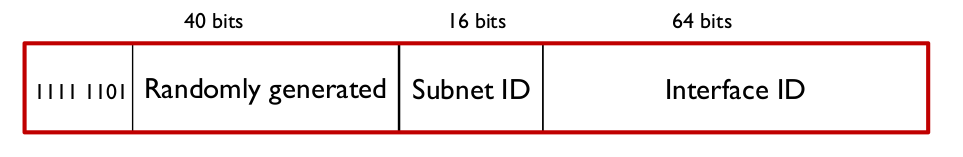
\includegraphics[width=1\textwidth]{indirizzo-unique-local.png}
    \caption{Indirizzo Unique Local}
    \label{fig:indirizzo-unique-local}
\end{figure}

\subsubsection{IPv4 Embedded Address}
Sono usati per rappresentare gli indirizzi ipv4 sugli indirizzi ipv6 e vengono messi nello spazion ::ff:0:0/80. Sono composti da:
\begin{itemize}
    \item i primi 80 bit a 0;
    \item 16 bit a 1;
    \item gli ultimi 32 bit rappreesntano l'indirizzo ipv4;
\end{itemize}

\subsubsection{Loopback Address}
L'indirizzo ::1 ha lo stesso scopo dell'indirizzo di loopback 127.0.0.1 di ipv4.

\subsubsection{Unspecified Address}
\`E un indirizzo unicast non specificato ::0, anche in questo caso il suo comportamento \`e lo stesso di ipv4.


\subsubsection{Indirizzi Anycast}
Ho degli indirizzi assegnati a dei nodi nelle rete e quando mando un pacche voglio che esso arrivi ad uno di essi (inizialmento pensato per i DNS server). Gli indirizzi anycast non sono utilizzati.


\newpage
\subsection{Protocolli IPv6}
In ipv6 alcuni protocolli sono stati integrati o rimossi rispetto ad ipv4, infatti ARP ed IGMP sono stati integrati in ICMP, la maggior parte degli altri protoccolli \`e stata fatta una modifica per supportare gli indirizzi a 128 ma le modifiche rimangono minime.

\subsubsection{IP}
L'header in ipv6 contiene molte meno dati che in ipv4, il motivo \`e che le informazioni sono presenti nel padding, tutto ci\`o \`e possibile grazie al campo next header. Si crea cos\`i una catena di header. Se non ho bisogno di estensioni allora il campo next header punter\`a all'header tcp.
\begin{figure}[H]
    \centering
    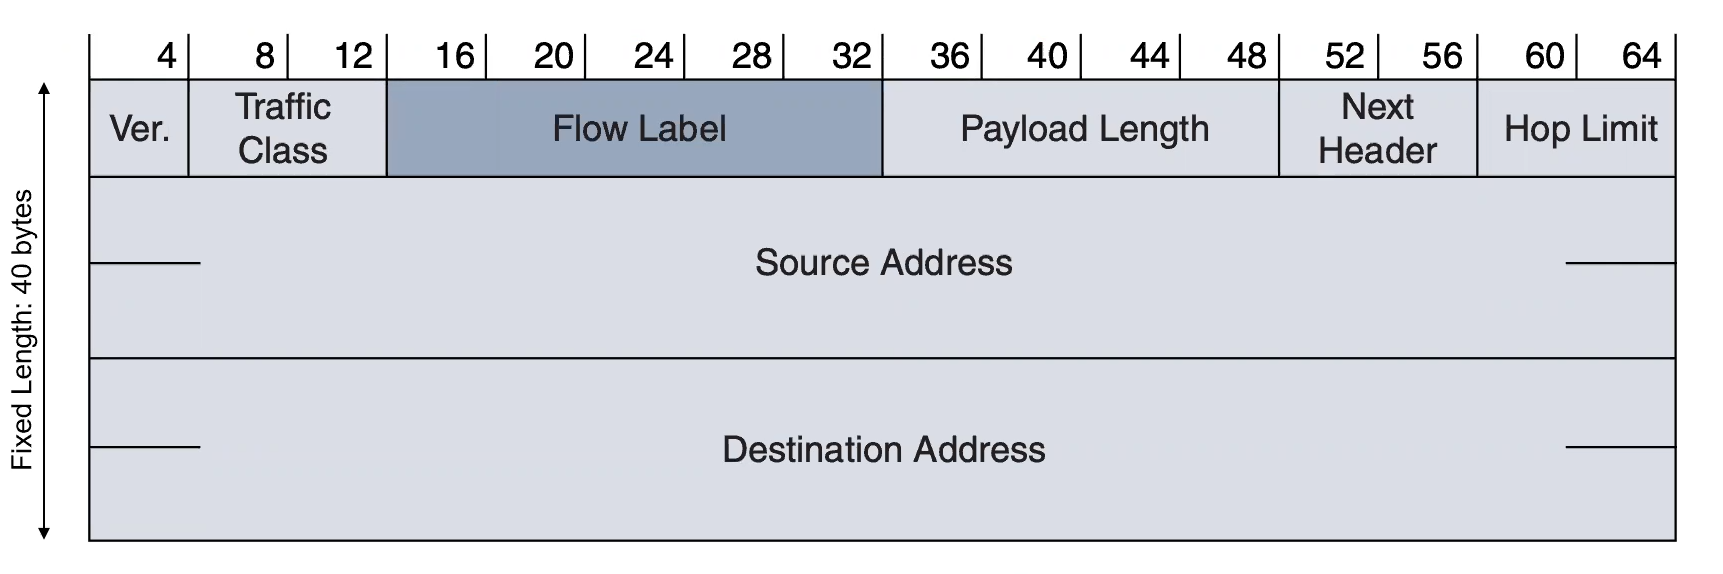
\includegraphics[width=0.8\textwidth]{ipv6-header.png}
    \caption{Ipv6 Header}
    \label{fig:ipv6-header}
\end{figure}
I campi rimasti sono:
\begin{itemize}
    \item ver: la versione del protocollo;
    \item traffic class: definisce delle classi di pacchetti per determinare delle priorit\`a tra i traffici degli utenti;
    \item flow label: etichetta associata al flusso, sar\`a possibile fare routing grazie a questo campo;
    \item payload lenght: lunghezza del payload;
    \item hop limit: time to live del ipv4;
    \item source address: indirizzo sorgente;
    \item destinatoin address: indirizzo destinazione;
\end{itemize}

\paragraph{Headers extensions}
Il protocollo utilizza dei codici per specificare quale sar\`a il campo dell prossima estensione.
\begin{figure}[H]
    \centering
    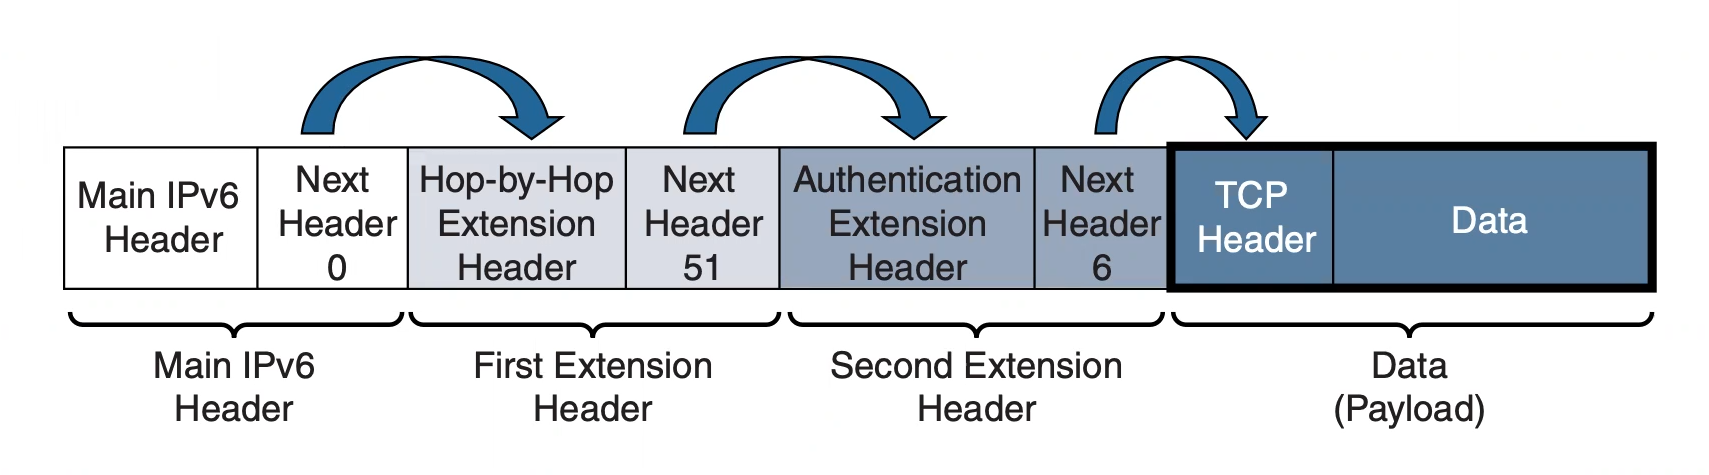
\includegraphics[width=0.8\textwidth]{header-chaining.png}
    \caption{Header Chaining}
    \label{fig:header-chaining}
\end{figure}
I diversi extension header hanno tutti gli stessi attributi:
\begin{itemize}
    \item next header code;
    \item lunghezza;
    \item extension data: dati relativi all'extension header;
\end{itemize}
Un estensione molto usata \`e la \textbf{Routing Extension Header}, dove viene specificata una lista di indirizzi su cui il pacchetto deve passare.


\subsection{Interfaccia con i livelli pi\`u bassi}
Nel livello 3 si \`e deciso di differenziare il protocllo ipv4 e ipv6 (approccio dual stack), infatti nel livello 2 esiste un campo che specifica il protocollo a livello superiore. Il \textbf{type} per ipv6 \`e 86DD.

\subsubsection{IPv6 Mutlicast Transmission}
\tolerance=1000
Quando si deve mandare un messaggio in multicast con ipv6 si utilizza una tecnica di mapping per creare un indirizzo MAC multicast appositamente per quetsto scambio di messaggi, il motivo \`e che si cerca di evitare l'utilizzo di un MAC broadcast address. I 32 bit bassi dell'indirizzo ipv6 multicast vengono mappati ai 32 bit bassi dell'indirizzo MAC, questo mapping viene specificato quando i primi 2 byte del MAC sono settati a 33:33, dunque un indirizzo MAC mappato sar\`a del tipo 33:33:xx:xx:xx:xx. Quando si manda un pacchetto all'indirizzo di broadcast ff0c::89:aabb:ccdd l'indirizzo MAC corrispondente sar\`a 33:33:aa:bb:cc:dd.

\subsubsection{Neigbhor Discovery}
Il protocollo ARP sar\`a sostituito dalla nuova version del protocollo ICMPv6. Quando si vuole mandare un pacchetto ad un host nella stessa sottorete e non si \`e a conoscenza del MAC, si utilizza il protocollo di neighbor discovery.

Il meccanismo di neighbor discovery avviene nel seguente modo: partendo da un indirizzo unicast si prendono i 24 bit bassi dell'indirizzo e si crea un indirizzo multicast solicited-node con i 24 bit bassi corrispondenti a quelli dell'unicast, questo permette quando si fa il mapping, di avere degli indirizzi MAC multicast che iniziano con 33:33:ff, grazie a come sono composti gli indirizzi solicited-node. In questo modo viene limitato il numero di pacchetti mandati nelle rete, la probabilit\`a che il pacchetto venga spedito all'host di destinazione \`e molto probabile, invece in ARP si mandava un pacchetto in broadcast a tutti gli host della sottorete.
\begin{figure}[H]
    \centering
    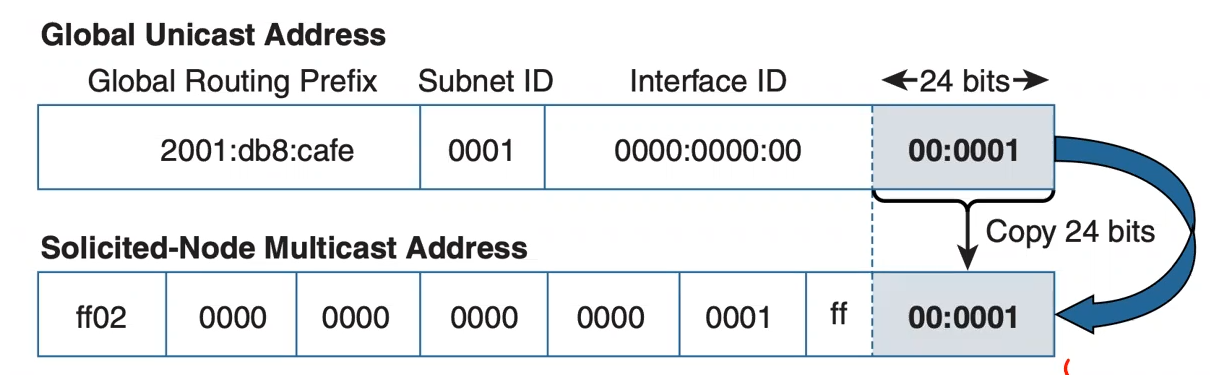
\includegraphics[width=0.8\textwidth]{solicited-node-multicast-address.png}
    \caption{Solicited Node Multicast Address}
    \label{fig:solicited-node-multicast-address}
\end{figure}

ARP:
\begin{itemize}
    \item manda un trama in broadcast;
\end{itemize}

Multicast:
\begin{itemize}
    \item manda a tutti;
    \item manda solo a chi fa parte di un gruppo: il MAC di multicast permette di mandare messaggi solo a chi appartiene a chi potenzialmente fa parte di quel gruppo;
\end{itemize}


\subsection{ICMPv6}
Il protocollo mantiene le opzioni di quello usato in ipv4 aggiungnendo delle funzionalit\`a per sostituire ARP e IGMP, ICMP \`e usato per:
\begin{itemize}
    \item diagnostica;
    \item neighbor discovery;
    \item multicast group;
    \item issue notification;
\end{itemize}

\subsubsection{Formato del messagio}
ICMP \`e incapsulto nel pacchetto ip.
\begin{figure}[H]
    \centering
    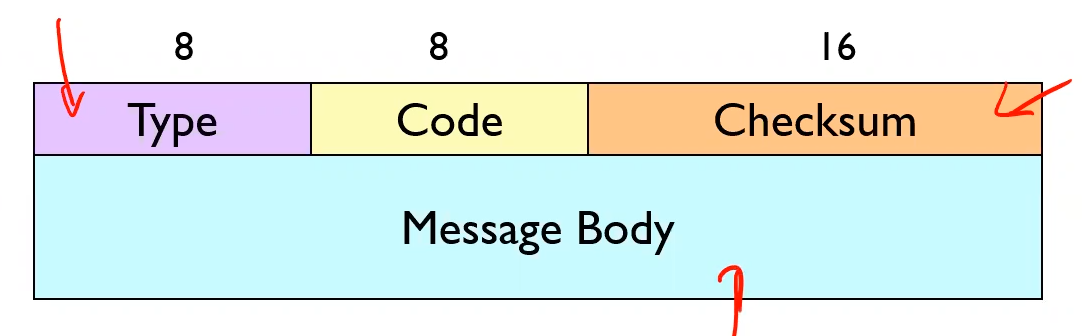
\includegraphics[width=0.8\textwidth]{icmp-format.png}
    \caption{Icmp Format}
    \label{fig:icmp-format}
\end{figure}
Messaggi di errore:
\begin{itemize}
    \item 1: destination unreachable;
    \item 2: packet too big;
    \item 3: time exeeded;
    \item 4: parameter problem;
\end{itemize}
Echo:
\begin{itemize}
    \item 128: echo request;
    \item 129: echo reply;
\end{itemize}

\subsubsection{Error Message}
\begin{figure}[H]
    \centering
    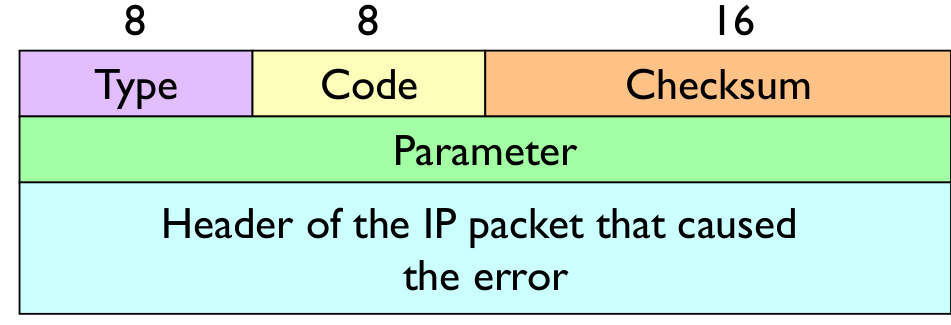
\includegraphics[width=0.8\textwidth]{icmpv6-error-message.png}
    \caption{Icmpv6 Error Message}
    \label{fig:icmpv6-error-message}
\end{figure}

\paragraph{Echo}
I messaggi di echo sono: echo request ed echo reply.

\subsubsection{Neighbor Solicitation}
Mandato da un host nella sotto rete.
\begin{figure}[H]
    \centering
    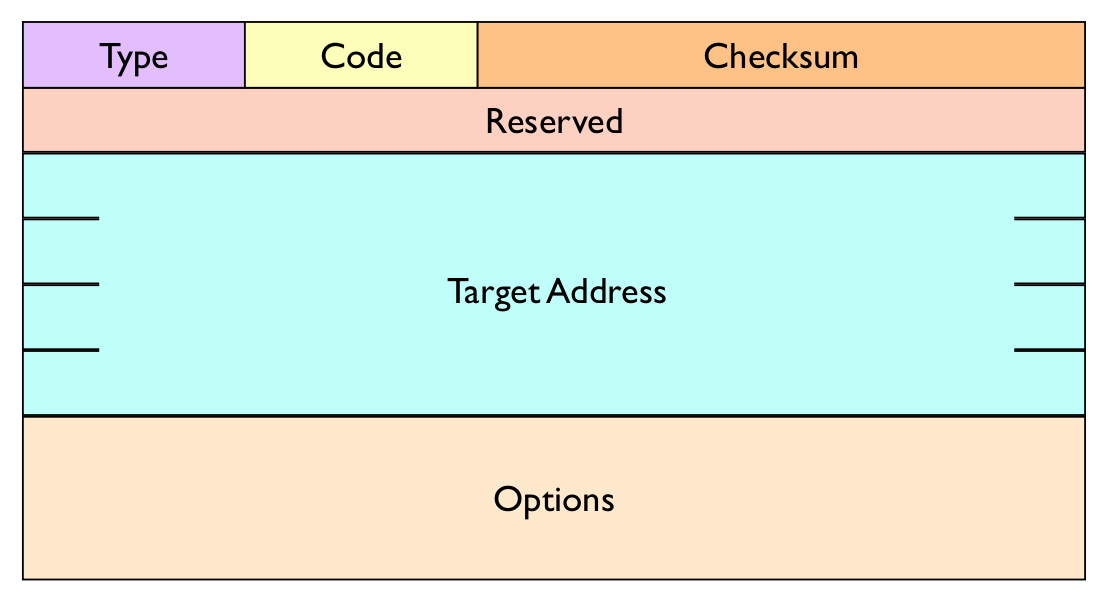
\includegraphics[width=0.6\textwidth]{neighbor-solicitation.png}
    \caption{Neighbor Solicitation}
    \label{fig:neighbor-solicitation}
\end{figure}


\subsubsection{Neighbor Advertisement}
Vengono aggiunti 3 flag nel campo reserved:
\begin{itemize}
    \item router: indica se il pacchetto arrivo da un router;
    \item solicited: specifica se il nodo \`e stato sollicitato o meno;
    \item override: specifice se l'host cache deve essere sovrascritta;
\end{itemize}
L'indirizzo MAC viene messo nel campo options, mentre l'ip di sorgente viene messo nel campo target address.

\subsubsection{Group Management}
Per gestire le comunicazioni multicast in un link local (sottorete) non si utilizza pi\`u il protocollo IGMP ma si usa ICMPv6, per gestire il join ai diversi gruppi si utilizzano tre tipi di messaggi:
\begin{itemize}
    \item Mutlicast Listener Query;
    \item Mutlicast Listener Report;
    \item Mutlicast Listener Done;
\end{itemize}
Un router inizia mandando un qeury a tutti gli host collegati utilizzando l'indirizzo ff02::1 (all host multicast address, solo host e non router), in questo modo vengono esposti i nodi che vogliono partecipare ad uno specifico gruppo. In teoria ha senso che tutti quanti gli host non appena ricevono la Query rispondano con la relativa Report, perch\'e in questo modo il router può avere la lista completa di tutti gli interessati. Ma nel tentativo di ottimizzare le trasmissioni, si \`e pensato che il router non dovesse possedere l’intera lista delle query con tutti i gruppi multicast, questo perch\'e il router dovrà semplicemente forwardare nella rete il pacchetto multicast quando è presente almeno 1 host nel gruppo multicast. \`E stato dunque inserito un timer randomico sugli host, che viene fatto partire quando viene ricevuta una query. Il primo host che manda un report viene registrato sia dal router che da tutti gli interessati al gruppo broadcast bloccando i loro timer.

Quando uno degli host si disconnette invia un Done. I router tengono un timeout per ogni entry nella loro tabella in caso un host si disconnetta senza inviare un done.




\subsection{Configurazione}
Le informazioni necessarie sono:
\begin{itemize}
    \item address prefix;
    \item interface id;
    \item default gateway;
    \item dns server;
    \item host name;
    \item domain name;
    \item MTU maximux transmission unit;
\end{itemize}
Per creare queste informazioni:
\begin{itemize}
    \item stateful config: informazioni date da un DHCP;
    \item stateless config: generate automaticamente;
    \item ibrida (stateless DHCP);
\end{itemize}

\subsubsection{Interface ID}
Si pu\`o configurare manualmente, ottenere dal DHCP oppure generati automaticamente. Nel modo di configurare i 64 bit bassi non si hanno garanzie che siano univoci, esiste un protocollo che permette il controllo e l'univocit\`a.

\paragraph{EUI-48 to EUI-64 Mapping}
\begin{itemize}
    \item EUI = Extended Unique Id
    \item OUI = Organization Unique Id
\end{itemize}
Per creare l'interface ID in modo automatico si pu\`o sfruttare la tecnica del mapping, si prende il MAC del interfaccia e viene mappato nel seguente modo:
\begin{figure}[H]
    \centering
    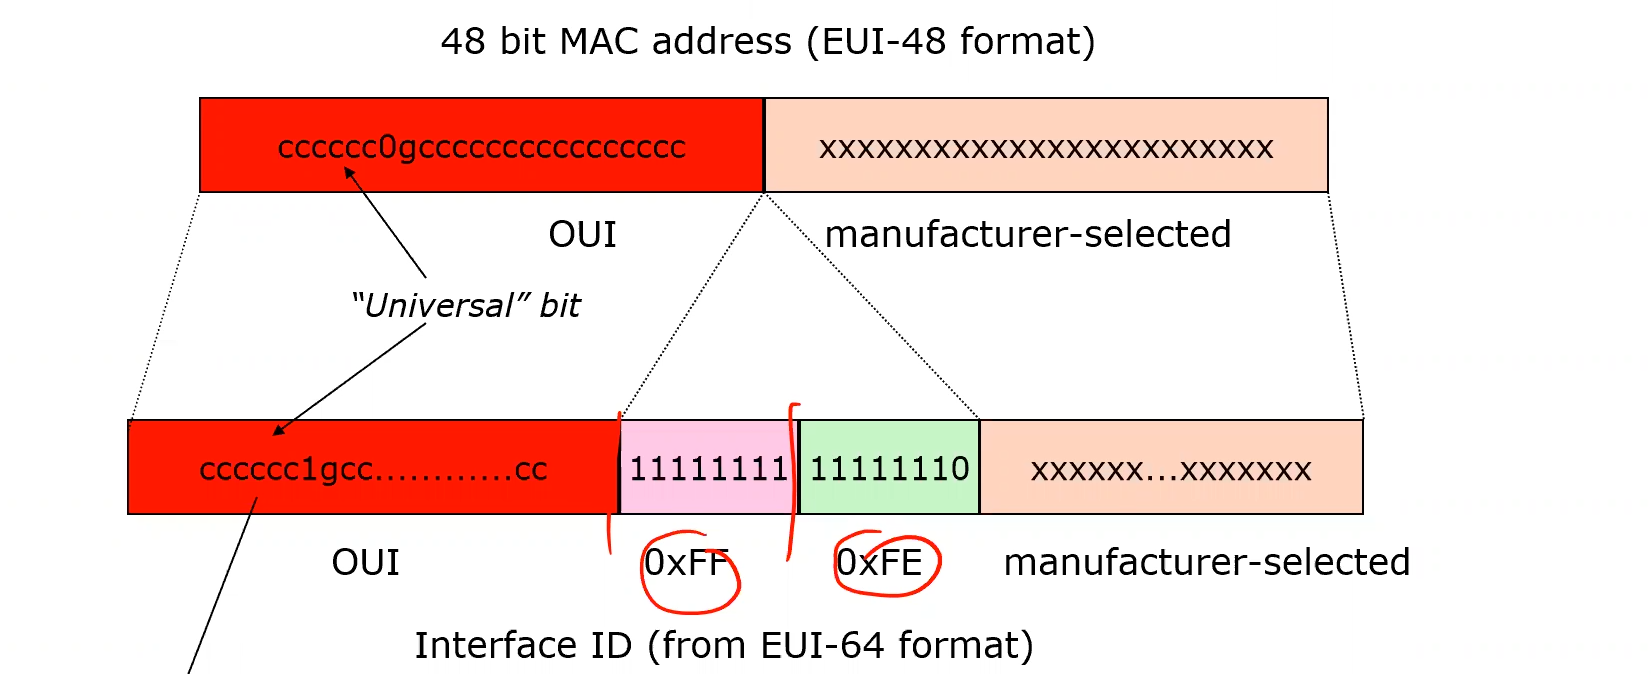
\includegraphics[width=0.8\textwidth]{mac-to-id-mapping.png}
    \caption{Mac To Id Mapping}
    \label{fig:mac-to-id-mapping}
\end{figure}
Il settimo bit viene settato a 0 il MAC \`e universale (la scheda di rete \`e configurata da un'organizzazione), mentre viene settato a 1 se il MAC \`e stato assegnato manualmente (quidni l'indirizzo sar\`a necessariamente univoco nella sottorete), questa \`e una convenzione ma non la regola.

\paragraph{Privacy Extension Algorithm}
Per evitare che l'interface Id possa essere calcolato da qualcun'altro ch conosca il MAC del mio dispositivo si usa un approccio per garantire maggior privacy ed aumentare la sicurezza.

Per generare l'interface Id si prendono 64 bit random e 64 bit generati del MAC mapping e poi viene fatto un hash. In fine il settimo bit viene settato a 0 perch\'e non si ha comunque la certezza che l'interface Id sia univoco.
\begin{figure}[H]
    \centering
    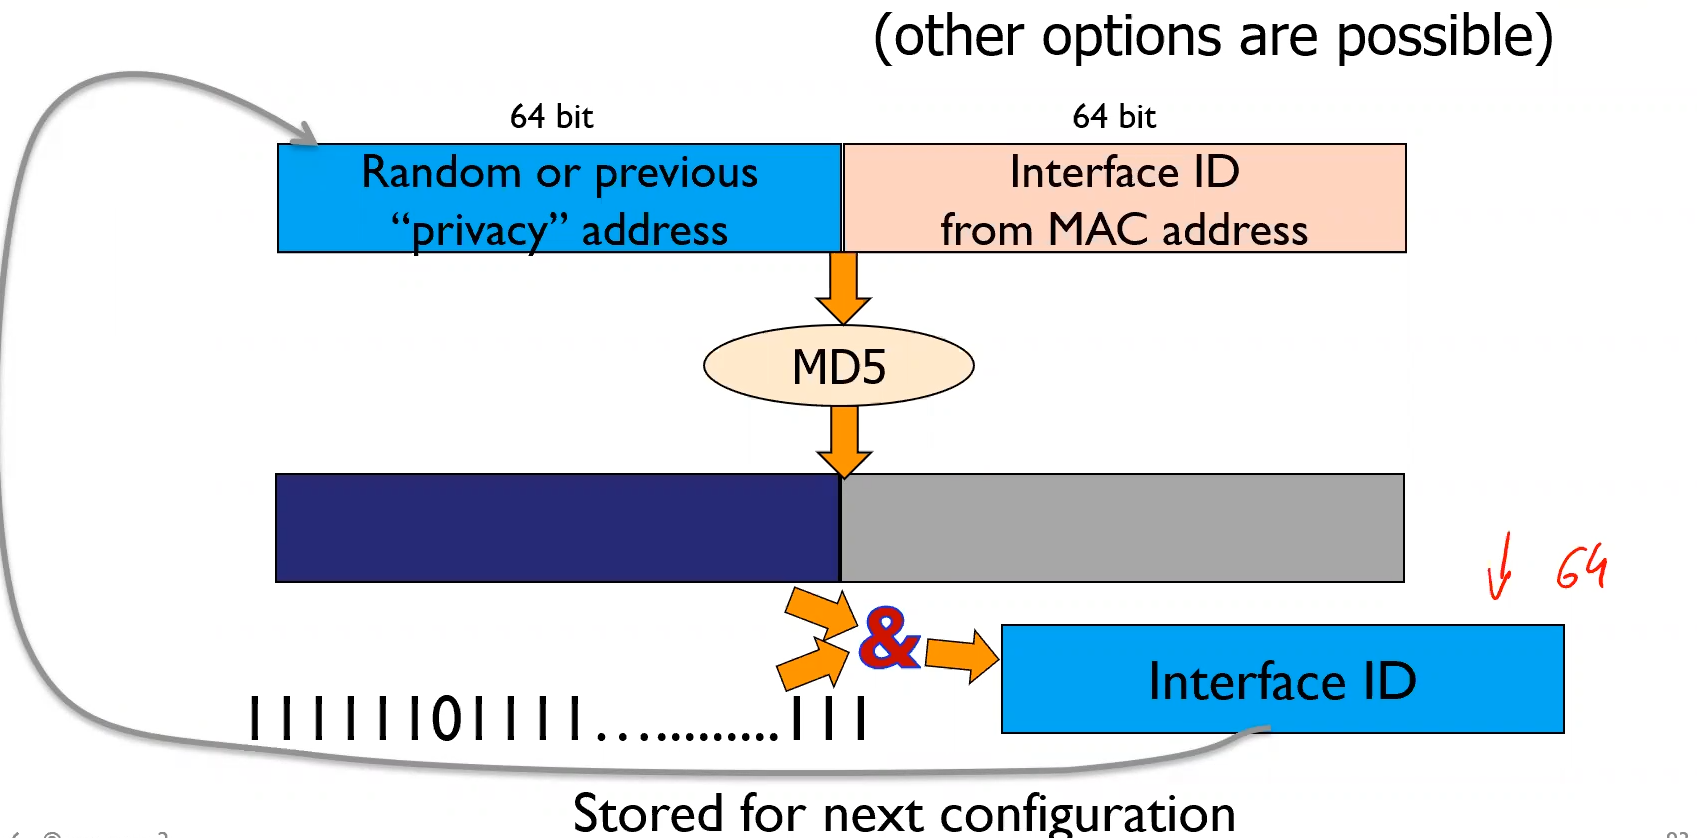
\includegraphics[width=0.8\textwidth]{privacy-extension-alogorithm.png}
    \caption{Privacy Extension Alogorithm}
    \label{fig:privacy-extension-alogorithm}
\end{figure}


\subsubsection{Address Prefix}
Anche in questo caso \`e possibile configurare la parte alta dell'indirizzo ip in modo manuale oppure in modo automatico. Per ottenere queste informazioni in modo automatico esistono due messaggi:
\begin{itemize}
    \item \textbf{Router Solicitation}: mandato a tutti i router con indirizzo multicast ff01::2.
        \begin{figure}[H]
            \centering
            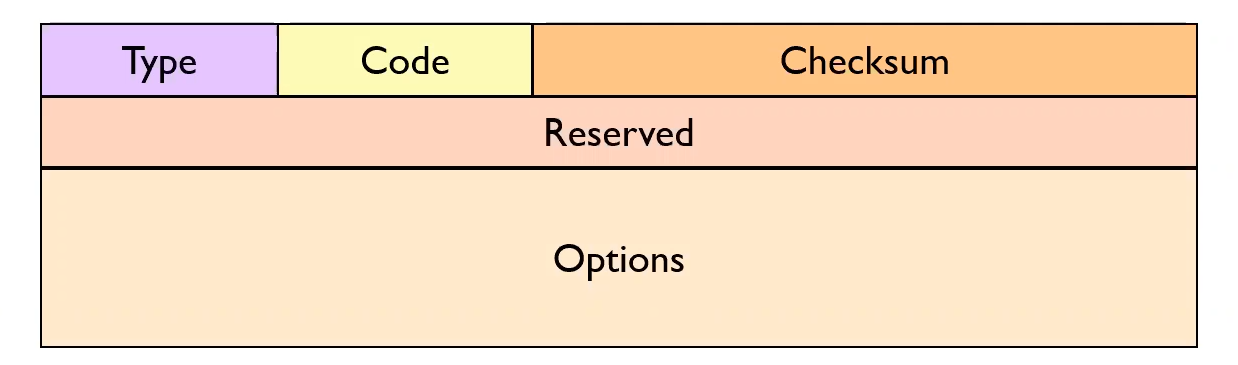
\includegraphics[width=0.8\textwidth]{router-solicitation.png}
            \caption{Router Solicitation}
            \label{fig:router-solicitation}
        \end{figure}
    \item \textbf{Router Advertisement}: pu\`o essere una risposa ad una solicitaion, M (Managed Address Configuration): se settato ad 1 indica che l'indirizzo \`e disponibile via DHCP; O (Other Configuration): parametri come il DNS server; Reachable Time: tempo in cui il router \`e disponibile; Retrans Timer: tempo in cui l'indirizzo \`e disponibile; solitamente l'indirizzo viene messo nel campo options;
        \begin{figure}[H]
            \centering
            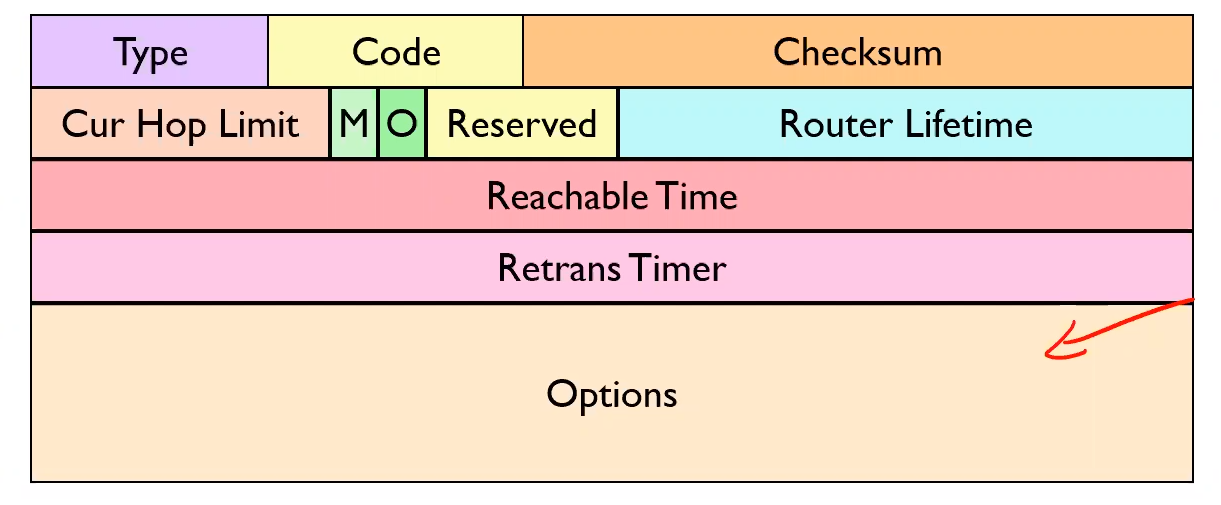
\includegraphics[width=0.8\textwidth]{router-advertisement.png}
            \caption{Router Advertisement}
            \label{fig:router-advertisement}
        \end{figure}
\end{itemize}
Quando un host si collega ad una rete potr\`a fare una solicitation e ricevere una advertisement oppure i router periodicamente mandano una advertisement.

\paragraph{Options}
Le opzioni hanno un loro formato particolare:
\begin{figure}[H]
    \centering
    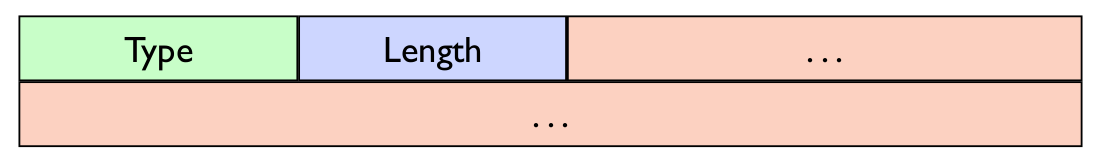
\includegraphics[width=0.8\textwidth]{options-format.png}
    \caption{Options Format}
    \label{fig:options-format}
\end{figure}
Le informazioni sul prefisso sono:
\begin{itemize}
    \item L: ad 1 se il prefisso pu\`o essere on-link;
    \item A: ad 1 se il prefisso pu\`o essere usato con una configurazione autonoma;
\end{itemize}
\begin{figure}[H]
    \centering
    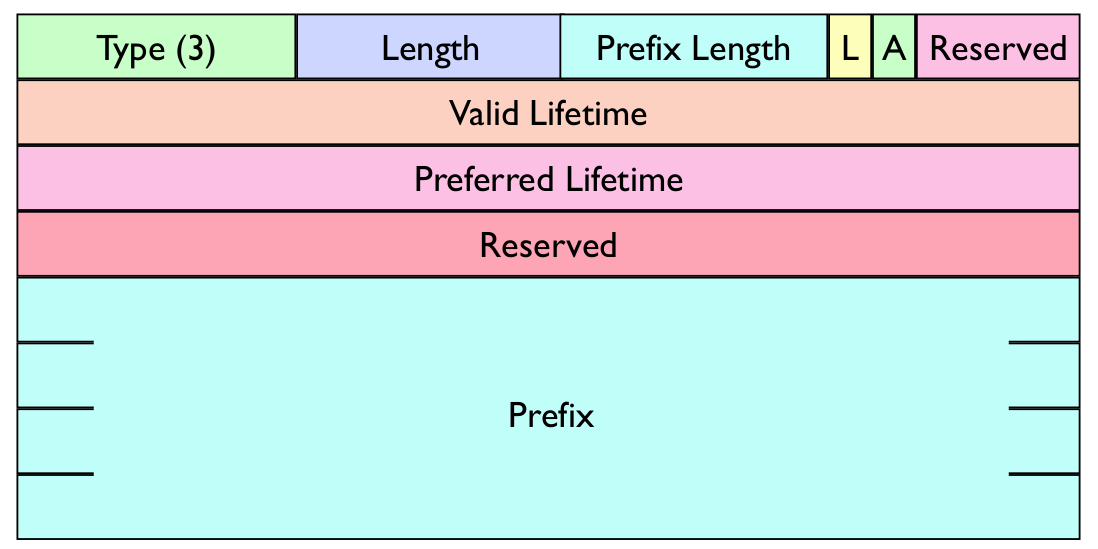
\includegraphics[width=0.6\textwidth]{prefix-information-options.png}
    \caption{Prefix Information Options}
    \label{fig:prefix-information-options}
\end{figure}

Un'altra opzione \`e il \textbf{Link Layer Address Option}, si mette il MAC del default gateway.

Un messaggio molto importante \`e l'\textbf{ICMP Redirect}, in una rete ci sono pi\`u router, l'host manda i pacchetti al suo default gateway, se per raggiungere un altro host un altro \`e router \`e pi\`u vicinino allora i pacchetti vengono rediretti in quel router.

\subsubsection{Duplicate Address Detection (DAD)}
L'host manda un messaggio di DAD ogni volta che viene effettuata una configurazione. Per verificare che non esistano indirizzi duplicati viene mandato una neghbor solicitation con l'indirizzo appena configurato, se un host ripsonde a questa richesta l'indirizzo viene cambiato.


\subsection{Stateless Config}
\begin{itemize}
    \item Il link local address viene generato automaticamente;
    \item successivamente viene fatta una DAD;
    \item l'host si iscrive al Solicited Node Multicast Address (configurando il MAC multicast e inviando una ICMP mutlicast listener report);
    \item abilita le comunicazioni on-link;
\end{itemize}

\subsection{Stateful Config}
\begin{itemize}
    \item viene inviata un router solicitation;
    \item si ascolta la router advertisement;
    \item si crea un indirizzo col prefisso annunciato;
    \item si prova la sua uncit\`a con la DAD;
    \item ci si iscrivi al solicitated node mutlicast address (configurando il MAC multicast e inviando una ICMP mutlicast listener report);
\end{itemize}

Un altra grosso vantaggio \`e il \textbf{Renumbering}, tramite l'advertisement si riassegnano gli indirizzi in modo automatico.


\subsection{Scope}
Qunado un dispositivo ha pi\`u interfaccie, gli indirizzi generati automaticamente saranno gli stessi, per distinguere le due interfacce l'host tiene conto a quale interfaccia mandare un messaggio. Per distinguere le due interfaccie si mette \%x, dove x \`e l'id dell'interfaccia.
\begin{figure}[H]
    \centering
    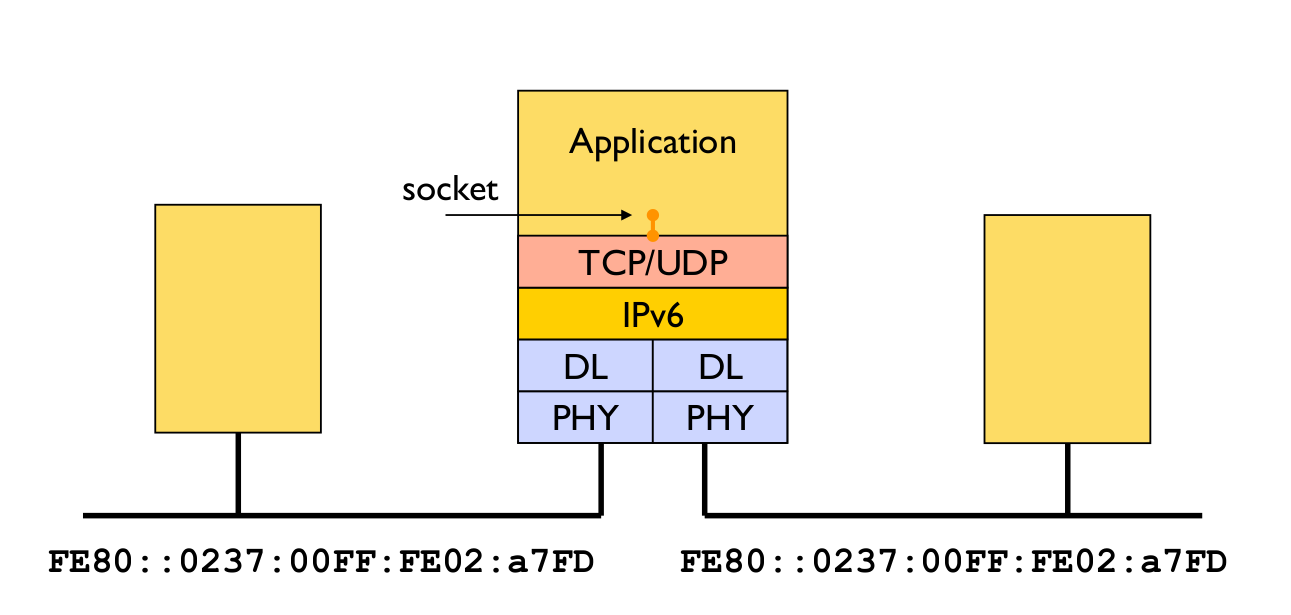
\includegraphics[width=0.8\textwidth]{ipv6-scope.png}
    \caption{Ipv6 Scope}
    \label{fig:ipv6-scope}
\end{figure}



\newpage
\section{IPv6 Transitioning}
IPv6 \`e ancora in via di utilizzo parziale, perci\`o si devono capire i problemi che sorgono nell'utilizzo di questo nuovo protocollo, si possono identificare 4 fasi di transizione, in cui IPv6 deventa incrementalmente pi\`u utilizzato fino a diventare lo standard:
\begin{itemize}
    \item \textbf{Network ipv6 isolati}: host di interfaccia dual stack, con ipv6 in ipv4 tunneling;
        \begin{figure}[H]
            \centering
            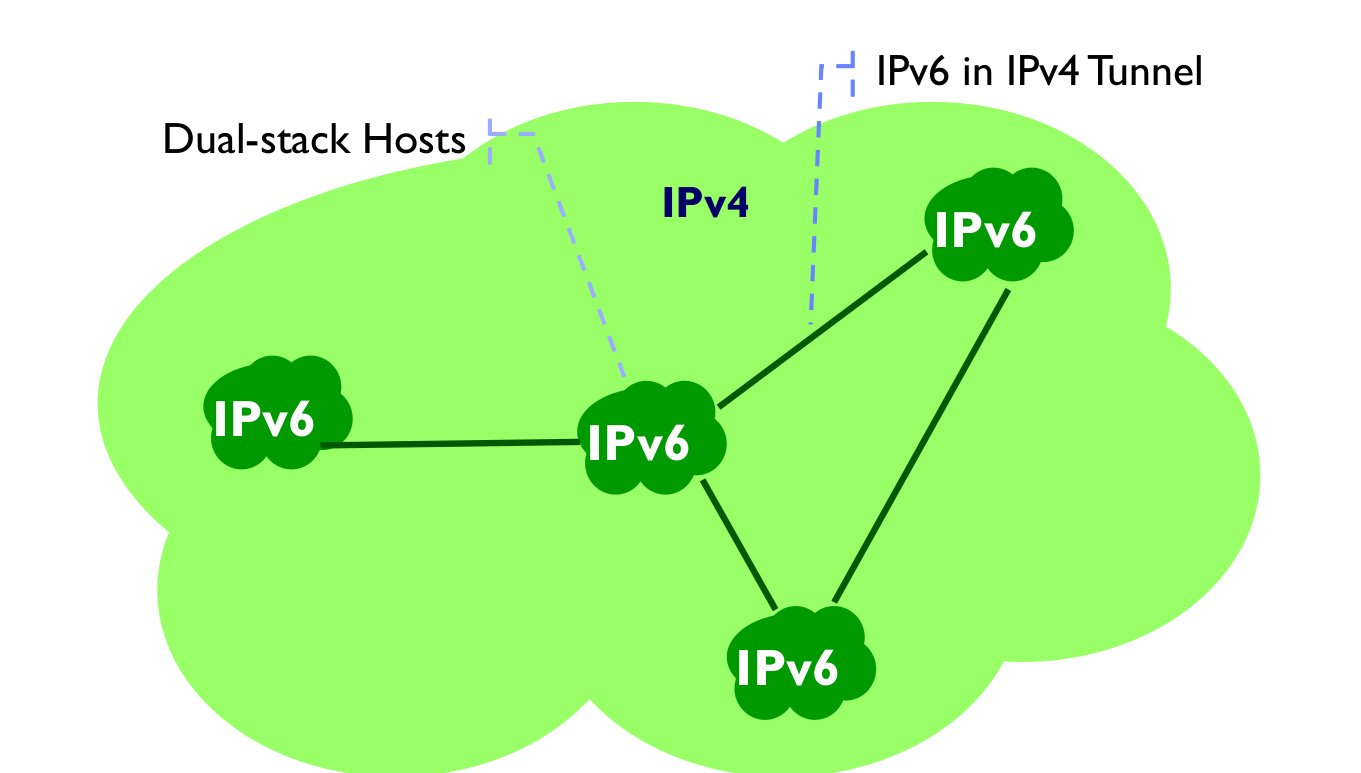
\includegraphics[width=0.4\textwidth]{isolated-ipv6.png}
            \caption{Isolated Ipv6}
            \label{fig:isolated-ipv6}
        \end{figure}
    \item \textbf{ipv6 island grow}: le isole diventano pi\`u grandi con soli host ipv6 all'interno, gli host di interfaccia sono dul stack translating devices;
        \begin{figure}[H]
            \centering
            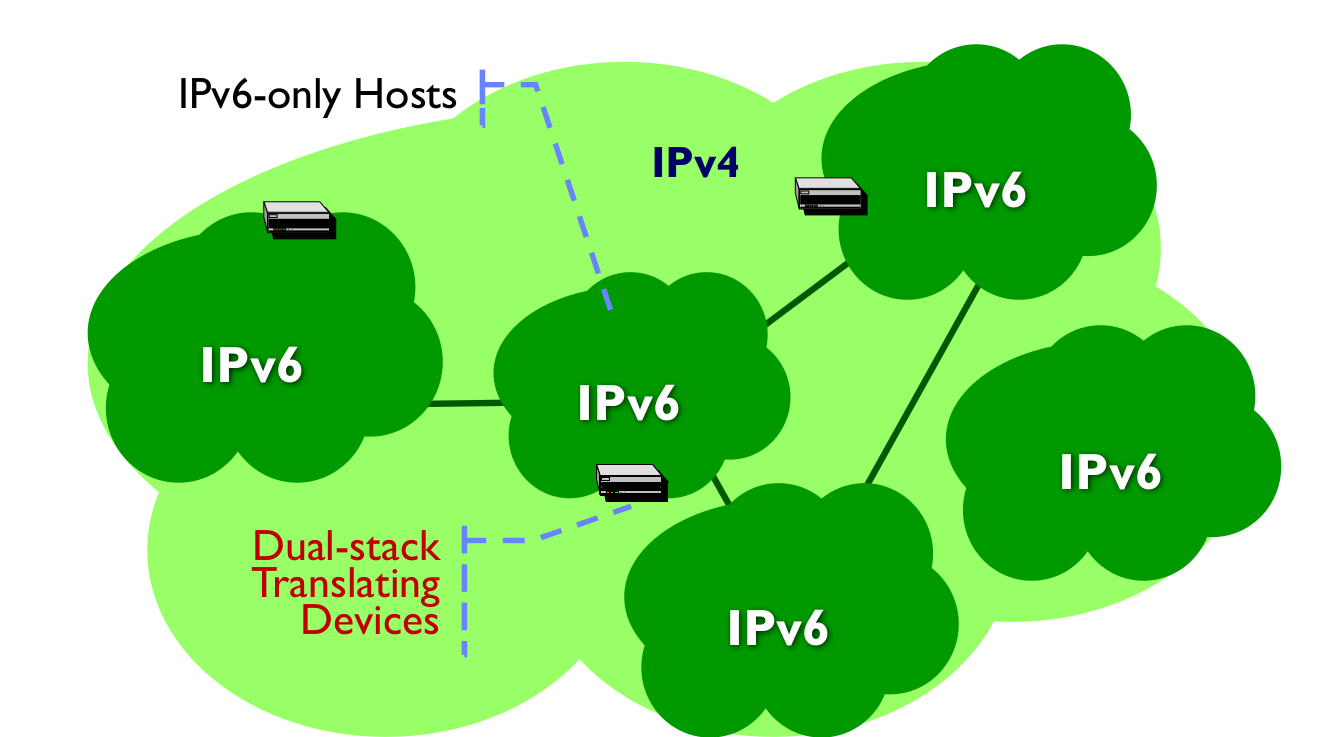
\includegraphics[width=0.4\textwidth]{ipv6-island-grow.png}
            \caption{Ipv6 Island Grow}
            \label{fig:ipv6-island-grow}
        \end{figure}
    \item \textbf{natice ipv6 connectivity};
        \begin{figure}[H]
            \centering
            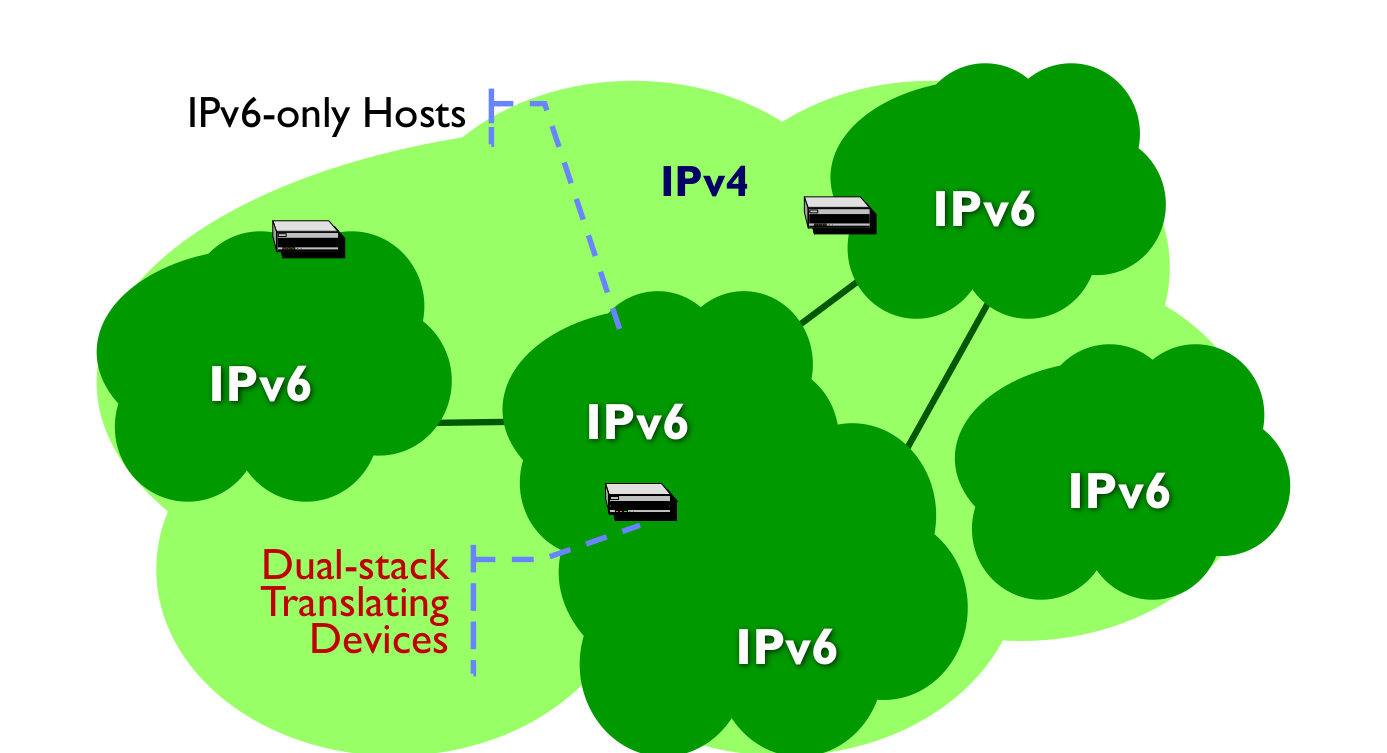
\includegraphics[width=0.4\textwidth]{native-ipv6-connectivity.png}
            \caption{Native Ipv6 Connectivity}
            \label{fig:native-ipv6-connectivity}
        \end{figure}
    \item \textbf{ipv6 takes over}: ipv4 isolati, ipv4 in ipv6 tunneling;
        \begin{figure}[H]
            \centering
            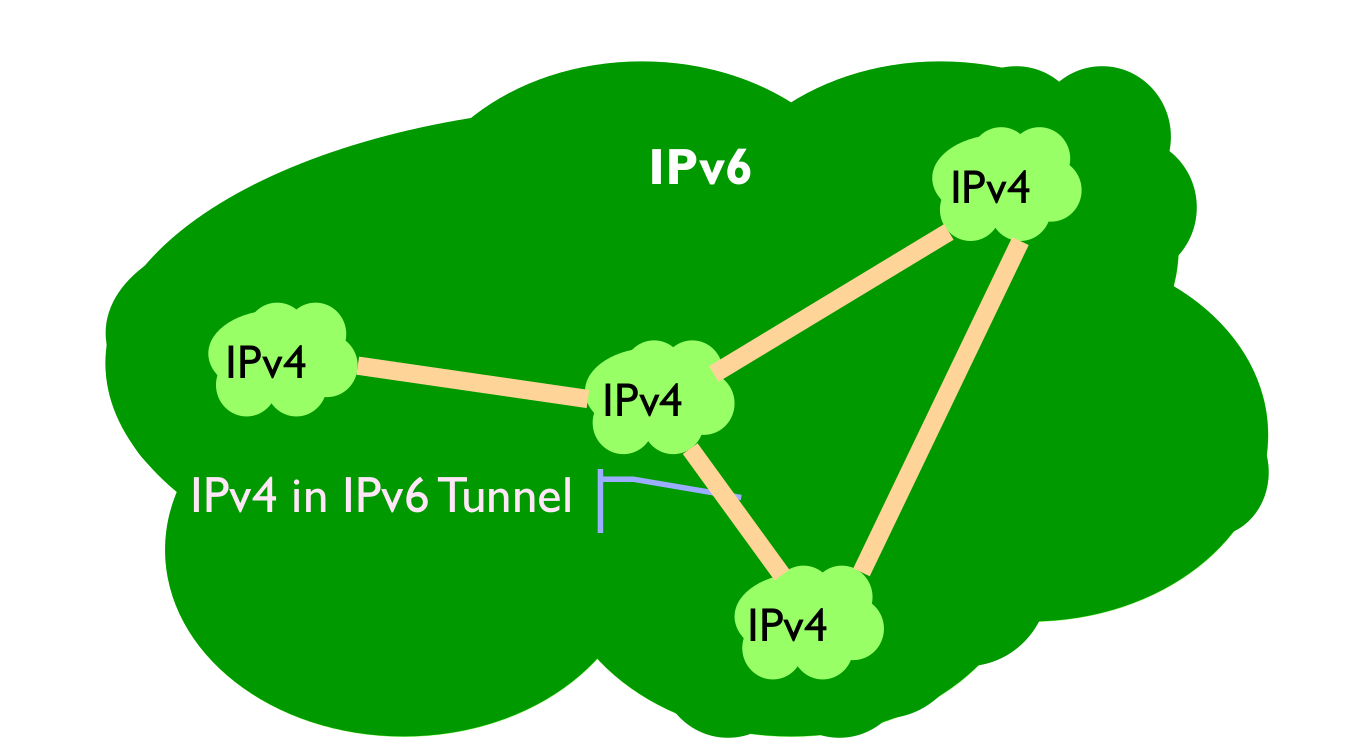
\includegraphics[width=0.4\textwidth]{ipv6-takes-over.png}
            \caption{Ipv6 Takes Over}
            \label{fig:ipv6-takes-over}
        \end{figure}
\end{itemize}


\subsection{Isolated IPv6 networks}
Si fa del \textbf{Tunneling}, partendo da un paccheto ipv6 che si interfaccia ad una rete ipv4, il router crea un header ipv4 e incapsula il pacchetto ipv6, il ricevitore con un indirizzo ipv4 dovr\`a poi riprendere il pacchetto ipv6 originale, per far in modo che questo avvenga i router devono essere necessariamente dual stack. Esistono dei vari protocolli che permettono di avere un mapping delgi indirizzi ipv6 algi indirizzi ipv4 automatico o manule.

Una di queste soluzioni \`e avare entrambi gli host in dual stack (\textbf{host-centered solutions}):
\begin{itemize}
    \item \textbf{IPv4-compatible addresses}: assegno solo degli indirizzi ipv6 compatibili con ipv4, quando devo inviare un messaggio a destinazione gli ultimi 32 bit dell'indirizzo ipv6 (::/96) sono i bit dell'indirizzo ipv4, dunque non ho conflitti;
        \begin{figure}[H]
            \centering
            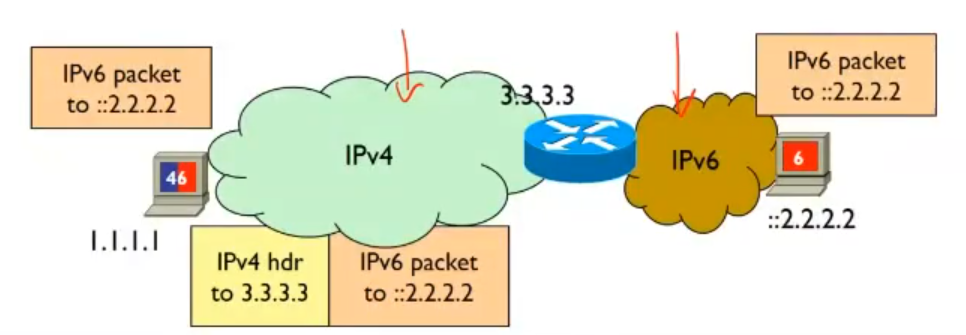
\includegraphics[width=0.5\textwidth]{ipv4-compatible-addresses.png}
            \caption{Ipv4 Compatible Addresses}
            \label{fig:ipv4-compatible-addresses}
        \end{figure}
    \item \textbf{6over4}: sfrutta il multicast dell'ipv4 e dell'ipv6, per\`o anche se in ipv4 \`e presente il multicast i provider non lo abilitano all'interno delle loro reti;
    \item \textbf{ISATAP}: l'ipv6 avr\`a su un prefisso comune (fe80::5efe) e gli ultimi 32 bit saranno dell'indirizzo ipv4;
    \item \textbf{neighbor discovery}: viene distribuita un lista dal DNS dove esistono i mapping tra indirizzi ipv4 e indirizzi ipv6, una delle limitazione \`e che ad ogni indirizzo ipv6 deve essere associato un hostname;
\end{itemize}

Posso avare anche delle soluzioni \textbf{network-centered}, dove esistono host nativi in ipv6 e degli host dual stack:
\begin{itemize}
    \item \textbf{6to4}: una delle principali limatazioni del mapping era il basso numero di bit utilizzati, allora una possibile soluzione \`e quella di andare a mettere l'indirizzo ipv4 nella parte alta dell'ipv6,
        \begin{figure}[H]
            \centering
            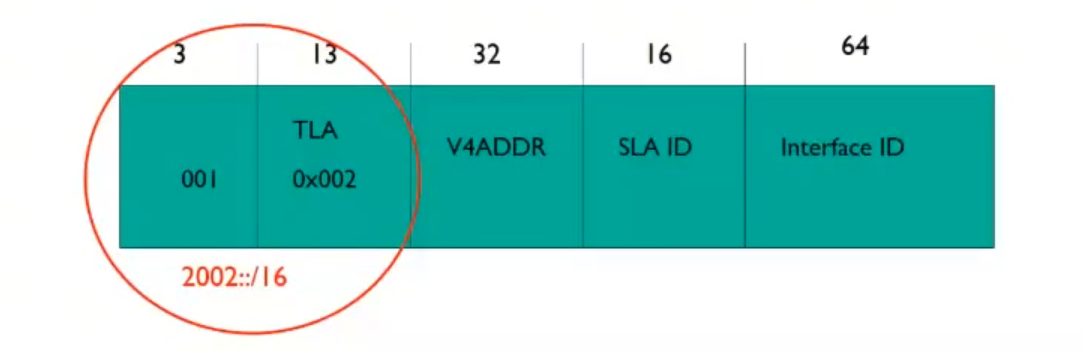
\includegraphics[width=0.6\textwidth]{6to4.png}
            \caption{6To4}
            \label{fig:6to4}
        \end{figure}
    \item \textbf{tunnel broker}: esiste un entit\`a nel mezzo che fa da broker per gli indirizzi da andare ad utilizzare per il tunnel;
\end{itemize}


Soluzioni \textbf{scalabili, carrier-grade solutions}, quando le isole ipv6 continuano a crescere si avranno anche scambi di pacchetti ipv4 attraverso reti native ipv6. Questo tipo di setup dovr\`a supportare ancora ipv4 clients e connessioni di host ipv6 a server in ipv4.

Il mapping di un indirizzo IP era proprio del NAT (map da ipv4 a ipv4), un dispositivo in grado di fare sia routing che natting viene detto Customer Permises Equipment (CPE). Alcune varienti del NAT \`e quello nelle reti cellulari, dove le antenne a cui si connettono il nat assegna un indirizzo publico all'host, per questo viene detta Large Scale NAT (LSN). Esiste anche un soluzione con entrambi gli approcci dove un LSN mappa delle reti private, in cui \`e presente il NAT per la traduzione. Alcune soluzioni di mapping tra indirizzi dipendono da dove viene inserito il NAT.
\begin{itemize}
    \item \textbf{AFTR (address family transmission router)}: grantisce agli host ipv4 di parlare con host ipv4 attraverso infrastrutture nel mezzo ipv6, l'AFTR tipicamente ha due funzionalit\`a: accalleratori hardware del nat e del tunneling;
    \item \textbf{Dual Stack Lite (DS lite)}: con questa soluzione si gestiscono tutti i casi in cui l'ISP abbia un backbone in ipv6, ds lite prevede che l'indirizzo ipv4 arrivi al CPE e che poi venga fatto un tunneling verso il Large Scale NAT (AFTR) e poi viene fatto il natting, lo svantaggio \`e che il piano di indirizzamento deve essere pubblico altrimente si potrebbero creare delle collisioni, le principali limitazioni sono: il NAT non \`e sotto il controllo del consumatore perch\'e un unico NAT gestisce tutti i clienti, il port forwarding non pu\`o essere abilitato nel CPR;
        \begin{figure}[H]
            \centering
            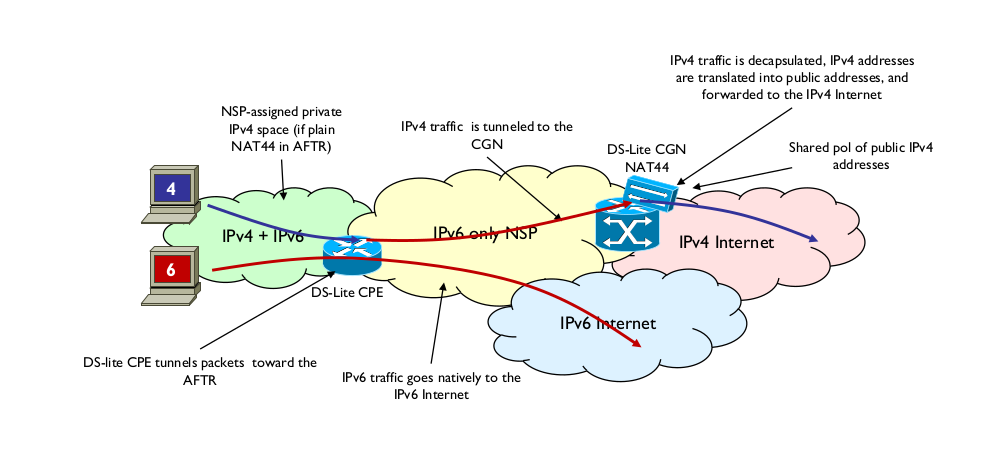
\includegraphics[width=0.8\textwidth]{ds-lite.png}
            \caption{Ds Lite}
            \label{fig:ds-lite}
        \end{figure}
    \item \textbf{A+P (address plus port)}: in questa soluzione rispetto a ds lite il NAT viene spostato dall'AFTR al CPR diventando sotto il controllo del consumatore, auemtando la scalabilit\`a, quando si manda un pacchetto in ipv4 passo da un indirizzo privato ad uno nattato e poi si fa un tenneling verso il AFTR, questo comporta l'assegnazione di un indirizzo ipv4 pubblico al CPR, il motivo \`e che quando si far\`a il natting \`e necessario avere un ip pubblico che si interfacci con la rete e che poi viene tunnelato. Se per\`o l'ISP ha scarsit\`a di indirizzi ipv4 si pi\`u utenti avrenno gli stessi indirizzi ip con dei range di porte diversi assegnati;
        \begin{figure}[H]
            \centering
            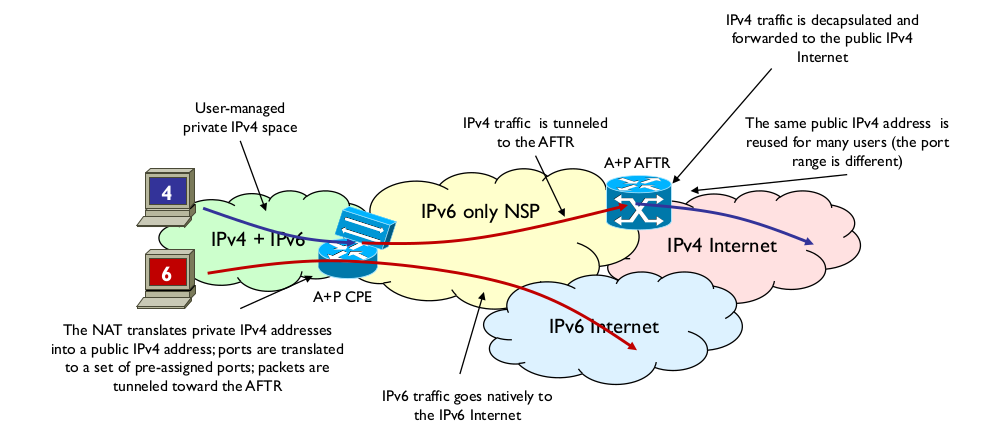
\includegraphics[width=0.8\textwidth]{a+p.png}
            \caption{A+P}
            \label{fig:a+p}
        \end{figure}
\item \textbf{MAP (mapping address and port)}: \`e un mix tra ds lite e a+p, in cui si tenta di avere una configurazione stateless, dove non si allocano dei range di porte al CPE, ma un set di porte, il vantaggio \`e che un border relay (AFTR) \`e in grado di ricostruire le informazioni a partire dall'indirizzo. Le caratteristiche sono:
    \begin{itemize}
        \item un client ipv4 viene mappato su un indirizzo univoco ipv6 caratterizzato dal prefisso del router CPE;
        \item l'indirizzo pubblico dell'host di destinazione viene mappato nel border relay;
        \item map-e: map con incapsulamento, il pacchetto ipv6 viene messo nel payload di un pacchetto ipv4;
        \item map-t: map con traduzione, in un pacchetto ipv6 l'header viene sostituito con un uno ipv4;
    \end{itemize}
    \begin{figure}[H]
        \centering
        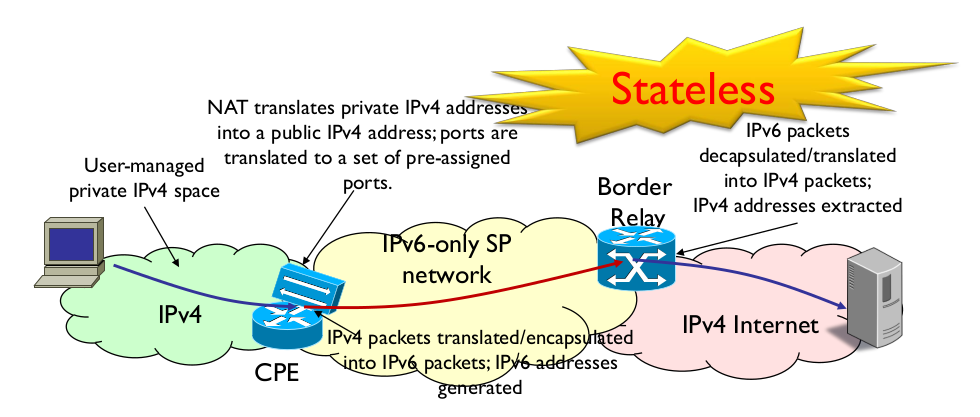
\includegraphics[width=0.8\textwidth]{map.png}
        \caption{Map}
        \label{fig:map}
    \end{figure}
    \begin{itemize}
        \item \textbf{Port set}: per generare i set di porte si utilizzano i 16 bit delle porte, ad ogni CPE veiene assegnato un PSID (Port Set ID) e un indirizzo ipv4 pubblico, ogni set di porte sono rappresetntate da: a bit maggiori di 0 (altrimenti si andrebbero a toccare le well-known ports), k bit di PSID, m bit (fino a 16 bit totali);
        \item \textbf{CPE ipv6 address}: si basa sul fatto che l'indirizzo ipv6 del CPE contiene delle informazioni sul CPE stesso e legate in qualche modo all'host ipv4 che ci vuole raggiungere, in modo che il border relay possa ricostruirsi l'indirizzo ipv6 a partire dall'indirizzo ipv4 da cui arrivano le risposte, perci\`o l'indirizzo si compone di:
            \begin{itemize}
                \item ruole ipv6 prefix: prefisso che indentifica l'istanza di map;
                \item EA bits: parte dell'indirizzo ipv4 pubblico e una porzione del port set;
                \item subnet id: compatibilit\`a con gli indirizzi ipv6 (sempre messi a 0);
                \item inteface id: informazioni dell'indirizzo ipv4;
            \end{itemize}
            \begin{figure}[H]
                \centering
                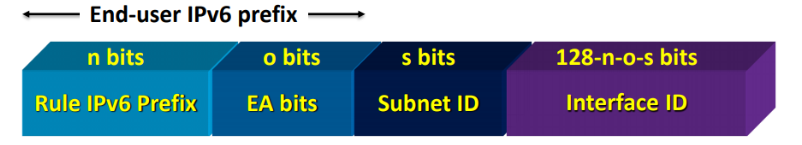
\includegraphics[width=0.8\textwidth]{cpe-ipv6-address.png}
                \caption{Cpe Ipv6 Address}
                \label{fig:cpe-ipv6-address}
            \end{figure}
        \item \textbf{map-e}:
            \begin{figure}[H]
                \centering
                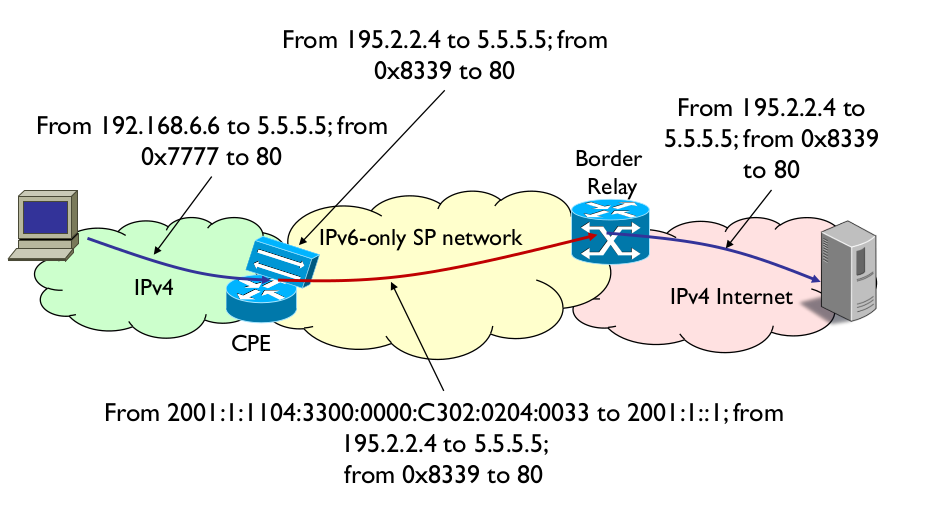
\includegraphics[width=0.8\textwidth]{map-e.png}
                \caption{Map E}
                \label{fig:map-e}
            \end{figure}
        \item \textbf{map-t}:
            \begin{figure}[H]
                \centering
                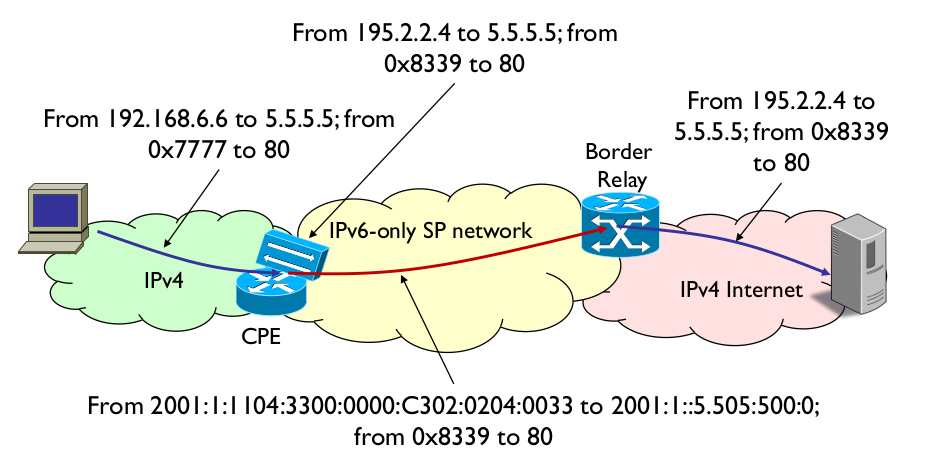
\includegraphics[width=0.8\textwidth]{map-t.png}
                \caption{Map T}
                \label{fig:map-t}
            \end{figure}
    \end{itemize}
    \item \textbf{NAT64 + DNS64}:  lo scenario \`e quando un client ipv6 vuole parlare con un indirizzo ipv4, questa operazione andr\`a fatta con un NAT64, l'indirizzo per\`o viene mappato dal DNS64. Per effettuare una risoluzione del nome, il DNS64 chiede a cui arriva una richiesta AAAA (ipv6) la inoltra al DNS del server ipv4 che risponde con un errore, allora il DNS64 manda una richiesta A (ipv4), il DNS6 mappa l'indirizzo ipv4 ricevuto ad un indirizzo ipv6 che inoltra al client, l'indirzzo ha un prefisso conusciuto (usato per le risoluzioni tradotte da ipv4) e la parte finale con l'indirizzo ipv4 del server, la richiesta che poi viene fatta passando per il NAT64 effettuer\`a una traduzione, creando l'header ipv4 a partire dall'indirizzo ipv4 dagli ultimi bit nell'indirizzo ipv6;
\end{itemize}



\newpage
\section{Wireless and Cellular Networks}
\subsection{Wireless LAN}
Le caratterisiche del link wireless sono:
\begin{itemize}
    \item un link Wireless ha un degrado maggiore del segnale, rispetta ad una fibra ottica;
    \item \`e soggetto a interferenze;
    \item problema del \textbf{fading}, causato dai rimbalzi del segnale su ostacoli;
\end{itemize}
Esistono vari standard dello IEEE 802.11 wireless LAN, i pi\`u moderni arrivano fino a 5GHz, il problema con le alte frequenze \`e 

Tutte le implementazioni utilizzano il protocollo di accesso \textbf{CSMA/CA}.

Un \textbf{access point} o una \textbf{base station} serve una \textbf{Basic Service Set (BSS)}, dentro la BSS si trovano sia gli access point che gli host.
\begin{figure}[H]
    \centering
    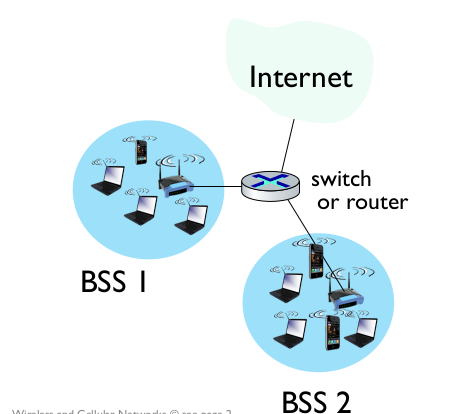
\includegraphics[width=0.6\textwidth]{bss.png}
    \caption{BSS}
    \label{fig:bss}
\end{figure}

Un dispositivo fa il \textbf{sensing} per cercare un canale operativo, che provengono di vari access point, ascoltando per il \textbf{beacon frame} che serve ad agganciarsi ad un access point, ci sono diversi beacon fram ed il dispositivo si collega all'access point con il segnale pi\`u forte, il beacon frame contiene:
\begin{itemize}
    \item il nome dell'AP (SSID);
    \item l'indirizzo MAC;
\end{itemize}
Per poter accedere ad una rete wifi, oggigiorno, hanno tutte bisogno di autenticazione, e tipicamente sar\`a presente un DHCP per ottenere una configurazione IP.

\subsection{CSMA/CA}
Il protocollo fa il sensing del canale (CSMA = carrier sense multiple access), ed la collision avoidance (CA), il motivo \`e che in una rete wireless il mezzo di trasmissione \`e l'aria che \`e un mezzo condiviso. 
Il sender:
\begin{itemize}
    \item si fa il sense del canale, si aspetta un tempo di DIFS e si trasmettono i dati;
    \item se si fa il sense ed il canale \`e occupato si aspetta, per applicare la CA parte un randon exponential backoff timer quando sento il canele occupato (in ethernet il timer partiva solo quando avveniva una collisione!);
\end{itemize}

Per evitare le collisione gli hots mandano un piccolo pacchetto , per sprecare la minor banda possibile, detti RTS (ready to send) usando CSMA, l'AP rispondono in broadcast agli host con un CTS (clear to send) per un degli host che ha mandato l'RTS, dopich\`e l'host a cui l'AP ha mandato il CTS che inizia a trasmettere una trama e l'AP manda sempre in broadcast un ACK all'host che ha trasmesso la trama.
\begin{figure}[H]
    \centering
    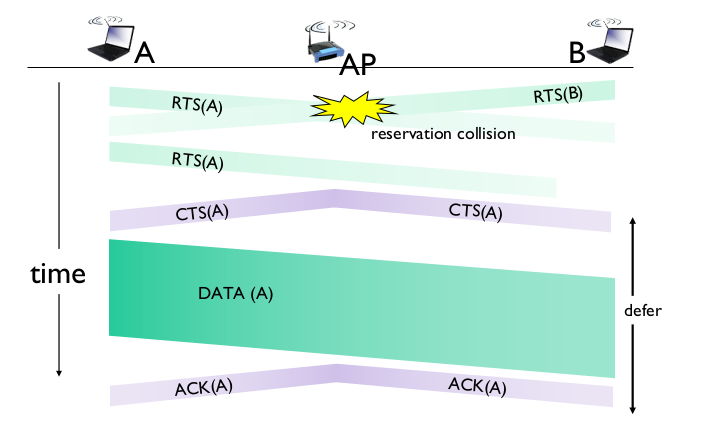
\includegraphics[width=0.8\textwidth]{collision-avoidance.png}
    \caption{Collision Avoidance}
    \label{fig:collision-avoidance}
\end{figure}

Una trama 802.11 \`e fatta da:
\begin{itemize}
    \item frame control: \`e composto da:
        \begin{itemize}
            \item protocal version;
            \item type: RTS, CTS, ACK, data;
            \item power mgt;
            \item ...;
        \end{itemize}
    \item duration: la durata che ci mette la trama per essere trasfertita;
    \item address 1: indirizzo dell'interfaccia MAC dell'AP, il motivo per cui \`e presente questo indirizzo \`e che nelle reti wireless bisogna prima passare dell'AP (violando in qualche modo il principio su cui si basa il livello link nelle reti ethernet, dove se uno swith \`e presente il pacchetto viene direttamente inoltrato al mac di destinazione, senza passare dal router);
    \item address 2: indirizzo sorgente;
    \item address 3: indirizzo dell'interfaccia del router a cui l'AP \`e collegato;
\end{itemize}
\begin{figure}[H]
    \centering
    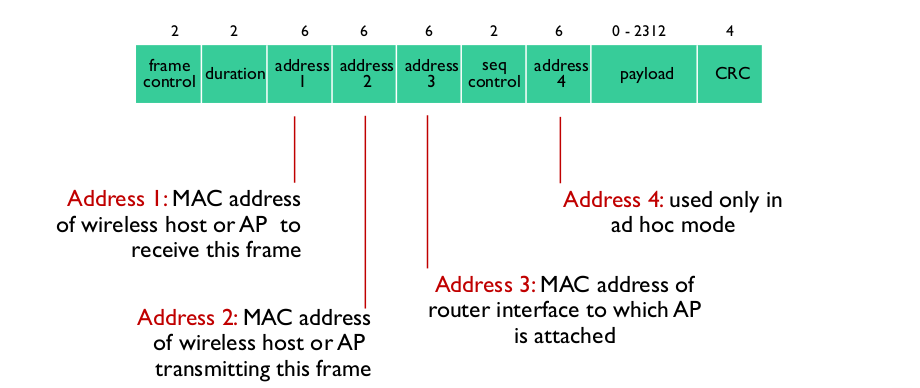
\includegraphics[width=0.8\textwidth]{802.11-frame.png}
    \caption{802.11 Frame}
    \label{fig:802.11-frame}
\end{figure}

In una rete wireless va gestita anche la mobilit\`a, questo \`e improbabile in una rete wifi, solitamente il movimento \`e fatto in una subnet, ovvero in una rete in cui sono presenti pi\`u AP collegati allo stesso router di una sottorete.

Un'altra capacit\`a dei dispositivi \`e il poter entrare in \textbf{sleep mode}, un nodo manda all'AP questa richiesta, se l'AP riceve delle trame da mandare al nodo li bufferizza finch\'e il nodo non si svelgia, un nodo si riattiva quando un beacon frame viene mandato, nel beacon frame vengono anche segnalati gli host per cui ci sono dei messagi in coda, allora il nodo capisce che deve svegliarsi e colleziona le trame, oppure continua a dormire.


\subsection{Cellular Networks}
Una rete cellulare \`e una rete che cerca di coprire un'area geografica molto vasta attraverso le \textbf{celle}, dove il terminale utente si muove anche su lunghe distanze, gestendo il cambiamento du una cella all'altra, detto \textbf{handover}.

La forma e le dimsioni di una cella sono determinate da:
\begin{itemize}
    \item potenza emessa;
    \item altezza;
    \item il guadagno dell'antenna: indica quanto un'antenna \`e buona nella trasmissione;
    \item morfologia del territorio;
    \item condizioni di propagazione: se nevica il segnale sar\`a pi\`u attenuato;
\end{itemize}
Le celle utilizzate in pratica sono:
\begin{itemize}
    \item Una \textbf{macrocella} viene relizzata con un'antenna posizionata molto in alto;
    \begin{figure}[H]
        \centering
        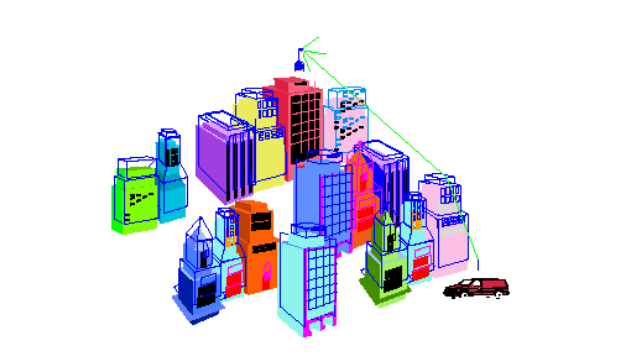
\includegraphics[width=0.6\textwidth]{macrocella.png}
        \caption{Macrocella}
        \label{fig:macrocella}
    \end{figure}
    \item \textbf{Microcella} realizzata con antenne non molto posta in alto,
    \begin{figure}[H]
        \centering
        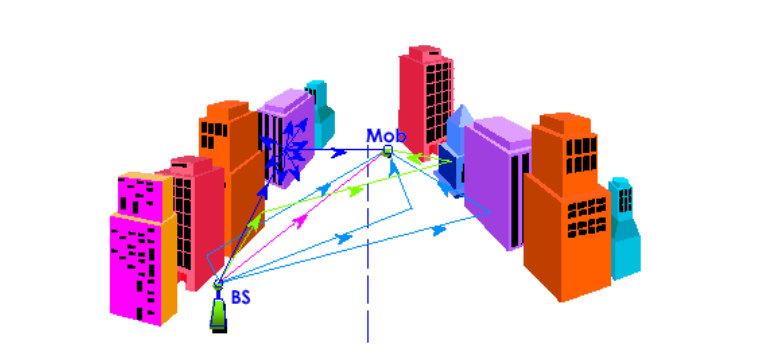
\includegraphics[width=0.6\textwidth]{microcella.png}
        \caption{Microcella}
        \label{fig:microcella}
    \end{figure}
\end{itemize}

Nelle reti cellulari non si usa CSMA/CD, le tecniche di condivisione sono: fdma, tdma, cdma, sdma. Per quasi tutte le reti cellulari si usa FDMA con riutilizzo dell frequenze, sfruttando la distanza fisica che separe le celle. Vengono creati dei \textbf{cluster} di celle in cui vengono usate tutte le frequenze disponibili, al di fuori di questo cluster si possono riutilizzare le frequenze, il numero di celle presenti in un cluster si indica con G=x. Nei cluster le celle che hanno le stesse frequenze si chimano \textbf{co-channel}.
\begin{figure}[H]
    \centering
    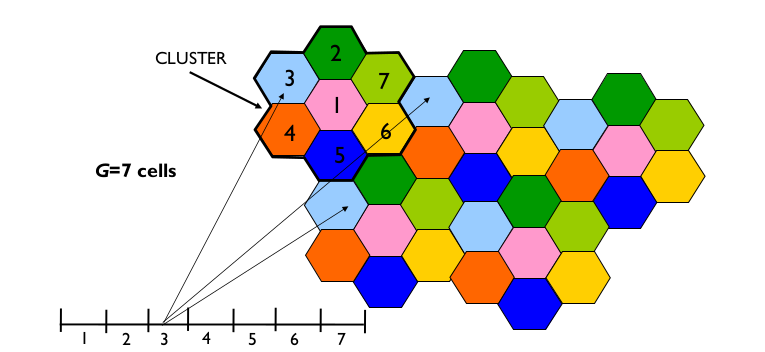
\includegraphics[width=0.8\textwidth]{7-cell-cluster.png}
    \caption{7 Cell Cluster (G=7)}
    \label{fig:7-cell-cluster}
\end{figure}
Per soddisfare pi\`u utenti si possono diminuire le dimensioni delle celle, soddisfando meno utenti per area ma incrementando l'ottimizzazoine di utilizzo delle frequenze, se per\`o si inzia a diminuire troppo la dimensione sorgono dei problemi:
\begin{itemize}
    \item aumento dei costi per creare le maggiori celle;
    \item diminuendo il numero di celle in un cluster aumento l'interferenza, la distanza tra i co-channel diventa pi\`u piccola, creando interferenze maggiori nella stessa frequenza;
\end{itemize}

Tecniche di freqency reuse:
\begin{itemize}
    \item \textbf{Splitting}: coesistenza di microcelle e macrocelle, esempio: in campagna sarebbe meglio gestita con macrocelle pi\`u copertura e meno persone da gestire, in citt\`a ha pi\`u senso usare delle micro celle, meno copurtura per pi\`u utenti da gestire e pi\`u ostacoli da evitare;
    \item \textbf{Cell Shaping}: per evitare degli handover mette le micro celle in posti dove le persone so che rimarranno ferme, e per le persone che si muvono avr\`o delle macrocelle che caoprono un area pi\`u ampia;
    \item \textbf{Power Control}: \`e una tecnica per evitare di sprecare pi\`u batteria del necessario, per decidere la potenza da utilizzare; le strategia sono: open loop, closed loop, ...; nell'open loop 
    \item \textbf{Sectoring}: si vanno a considerare delle antenne con capacit\`a di trasmissioni non omnidirezionali, diminuendo le interferenze in una certa direzione;
    \item \textbf{Tilting}: non usare un angolo di 90 gradi per le trasmissioni, limitando le interferenze;
    \item \textbf{Creating femtocell}: si creano delle celle al volo quando ne ho bisogno dove ne ho bisogno, esempio: uno stadio non avrebbe senso di essere gestito ogni giorno della settimana, se non quando lo stadio si riempe di gente per un evento;
\end{itemize}

jArchittura ...

\subsection{Basi Procedures}
\begin{itemize}
    \item \textbf{Registrazione}: fornire un associazione ad un rete cellulare, la registrazione viene fatta ogni qual volta un utente voglia accedere ad un servizione;
    \item \textbf{Mobilit\`a}: le procedure legate alla mobilit\`a sono:
        \begin{itemize}
            \item \textbf{Roaming}: il roaming \`e la capacit\`a di un terminale di essere tracciabile in una rete, tenendo i log su ogni cella in cui \`e stato attaccato. Per effettuare il roaming la rete ricorda in quale location area il terminale si trova, pi\`u celle adiacenti formano una lacation area, non \`e detto che una location area sia fatta da celle di un solo opertatore. Ognuna di queste lacation area ha un ID detto Location Area Id (LAI);
            \item \textbf{Location updating}: \`e l'operazione che un utente deve fare ogni qual volta si muove e cambia location area, un treminale si accorge di aver cambiato LA quando visualizza un LAI diverso;
            \item \textbf{Paging}: come si fa ed essere tracciabili? La rete conosce la LA in cui il terminale si trova, ma non la specifica cella, allora quando arriva un messagio per host x, il sistema manda un \textbf{paging message} in broadcast in tutta la LA (simile ad un ARP request), il motivo per cui si manda un messaggio in broadcast in una location area \`e limitare il numero delle laction updating;
            \item \textbf{Handover}: procedura molto complessa per continuare a mantenere la connessione passando da una cella all'altra, si classificano in: intra-cella vs inter-cella, (soft vs hard) sono collegato ad entrambe le base station, sono collegato prima ad una e poi ad un altra, (MT vs BS) inizializzata da MT a dalla BS (tipicamente), (Backward vs Forward) procedure gestite dalla cella di arrivo o dalla cella di partenza;
        \end{itemize}
\end{itemize}

\subsection{Evoluzione delle reti cellulari}
La prima generazione (1G) era una tecnologia completamente in analogico in FDMA, sostitutita dal \textbf{GSM (Europa) 2G}, in europa adottato con FDMA/TDMA, il passo in avanti \`e stato il passaggio dall'analogico al digitale e l'avvento degli sms, con il \textbf{2.5G GPRS/EDGE} \`e la prima tecnologia di fornire srevizi a pacchetti.

\textbf{3G} dove il focus \`e improntato al miglioramento dello scambio di contenuti multimediali, che adotta il CDMA in USA, UMTS in Europa. L'estensione del \textbf{3.5G}, va a migliorare l'UMTS che diventa HSPA aumentando di fatto la grandezza dei dati scambiati.

\textbf{4G} conosciuto comee LTE, ha un focus sul creare un'architettura ben integrata con i servici TPC/IP forniti da internet, vengono create delle antenne MIMO in cui si riesce a trasmettere su pi\`u canali in contemporanea, aumentando di molto il bitrate. Per la volta la rete \`e interamente in IP, anche per chiamate vocali.

\textbf{5G} cerca di unificare diverse tecnologie di accesso wireless, di fatto annullando le diversit\`a tra rete cellulare e wifi. Il 5G utilizza delle \textbf{mmWave} (micro onde) permettono di avere un throughput maggiore. Si cerca di offrire dei servigi aggiuntivi come l'\textbf{edge computing}, spostando le computazione da un server ad dei nodi vicini alla BS, cercando di fornire dei servizi personalizzati attraverso la virtualizzazione dei servizi di rete (come ad esempio un firewall), detto \textbf{NFV (Network Function Visualization)}. Queste funzioni di rete vengono combinate in una catena di rete, utilizzando anche il source routing di ipv6. Esiste anche l'\textbf{SDN (Software Define Networking)}, serve per eseguire tutte queste funzioni ho bisogno di un disallineamento tra piano di controllo e piano dati, il router avr\`a bisogno di un sitema general purpose per poter gestire questi due servizi in modo differente, gestendo in maniera opportuna la catena di servizi.

\subsection{GSM}
Offre servizi come:
\begin{itemize}
    \item voce a (13 kbit/s o 6.5 kbit/s);
    \item sms;
    \item servizi supplementari;
\end{itemize}
L'architettura GSM \`e fatta da:
\begin{itemize}
    \item \textbf{Mobile Station}: si tratta di dispositivi in grado di connettersi;
    \item \textbf{Subsrciber Identity Module (SIM)}: per connetersi alla rete, il dispositivo ha bisogno di una sim, che contiene dei parametri per autenticazione e di altri dati, uno di questi \`e l'IMSI che \`e molto simile ad un MAC, il dispositivo + sim formano un \textbf{mobile terminale (MT)};
    \item \textbf{Base Station Subsystem (BSS)}: la BS \`e formata da una Basa Transceiver Station BTS che \`e in grado di modulare su pi\`u frequenze i diversi canali di accesso, e da una Base Station Controller BSC, che gestisce tutta la logica delle rete, come ad esempio la gestione dall'handover, manda inoltra il segnale di paging per localizzare un utente, e converte i 13kbit per la voce a 64kbit/s (il motivo \`e perche\'e la rete cellulaure usa PCM64);
    \item \textbf{Network and Switching Subsystem (NSS)}: la BSS \`e collegata a:
        \begin{figure}[H]
            \centering
            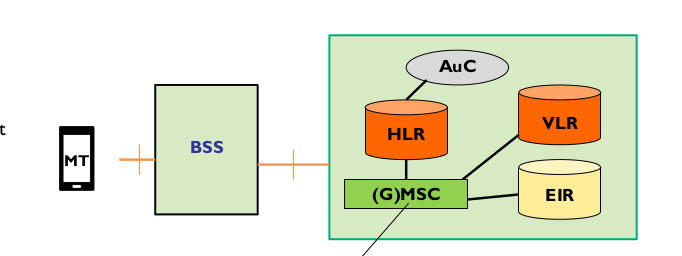
\includegraphics[width=0.6\textwidth]{nss.png}
            \caption{Nss}
            \label{fig:nss}
        \end{figure}
        \begin{itemize}
            \item MSC (Mobile Switching Center): gestisce l'autenticazione, il routing tra il GSM ed altri network;
            \item HLR (Home Location Register): \`e il database della rete a cui appartiene il dispositivo home, nella quale vengono registrati i parametri dell'utente, come le chiavi crittografiche, dati di mobilit\`a, \`e unico per tutta la rete;
            \item VLS (Visitor Location Register): contiene le informazioni legati ad un MT presente in quel momento nella rete, mantiene i valori quando l'utente si \`e spostato;
            \item AuC (Authentication Center): tramite una tecnologia challange and response, l'utente si pu\`o autenticare;
            \item EIR (Equipmente Identity Register): mantiene un registro di tutti i dispositivi rubati;
        \end{itemize}
    \item \textbf{GMS Frequenze}: le frequenze allocate al GMS sono: 850, 900, 1800, 1900 MHz. Le frequenze in uplink sono diverse da quelle in downling;
    \item \textbf{Canali}: si usa un approccio FDMA/TDMA, la divisione \`e in 32 frequenze portanti, inoltre ogni canale viene diviso in 8 slot temporali. All'interno degli slot le informazioni vengono arganizzate in burst:
        \begin{figure}[H]
            \centering
            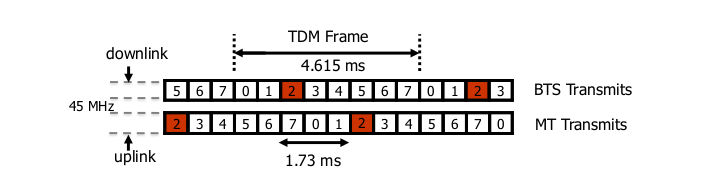
\includegraphics[width=0.6\textwidth]{up-down-link.png}
            \caption{Up Down Link}
            \label{fig:up-down-link}
        \end{figure}
    \item \textbf{Timing Advance}: ci sono dei ritardi di propagazione, comportando dei problemi con la trasmissione negli slot assegnati, per questo viene usato il timing advance, misurando i ritardi di propagazione si inizia a trasmette con un anticipo temporale pari a al ritardo di propagazione, infatti all'inizio e alla fine del burst sono presenti dei bit inutili, detti di guardia, per evitare sovrapposizioni con gli altri cananli, anche per problemi di disallineamento;
    \item \textbf{Struttura burst}:
        \begin{figure}[H]
            \centering
            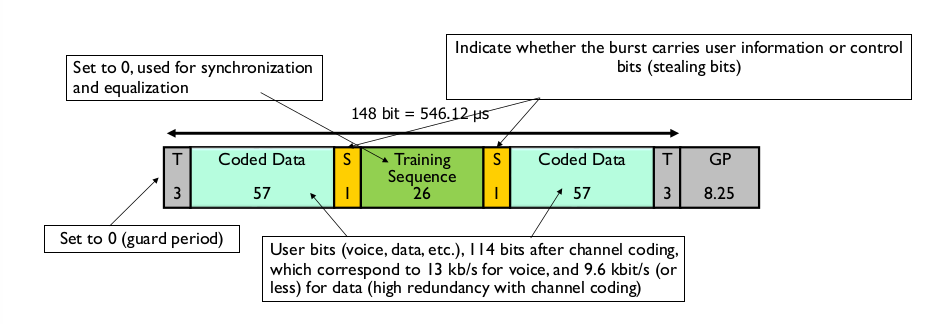
\includegraphics[width=0.6\textwidth]{struttura-burst.png}
            \caption{Struttura Burst}
            \label{fig:struttura-burst}
        \end{figure}
    \item \textbf{Canali Logici}: i canali logici sono mappati sui canali fisici che identificano cosa viene trasmesso all'interno dei canali, divisi in traffic channel e control channel.
\end{itemize}

\subsection{LTE}
Una delle caratterisiche principali \`e il rimpiazzamento del CDMA con l'FDMA (OFDMA: FDM dove le frequenze portanti sono pi\`u vicine tra di loro ed ortogonali tra di loro).

L'LTE \`e composto da:
\begin{itemize}
    \item LTE utilizza 3 diverse bande di frequenza:
        \begin{itemize}
            \item 2600 MHz per citt\`a;
            \item 1800 MHz medio gittata;
            \item 800 MHz lunghe gittate, pochi utenti, pochi ostacoli;
        \end{itemize}
    \item \textbf{Terminologia}:
        \begin{itemize}
            \item \textbf{downling (DL)}: 
            \item \textbf{upling (UL)}:
            \item \textbf{User plane}:
            \item \textbf{control plane}:
        \end{itemize}
    \item \textbf{Architettura}: \`e formata da RAN Radio Access Network, ... ,  le BSS vengono chiamate eNodeB, 
        \begin{figure}[H]
            \centering
            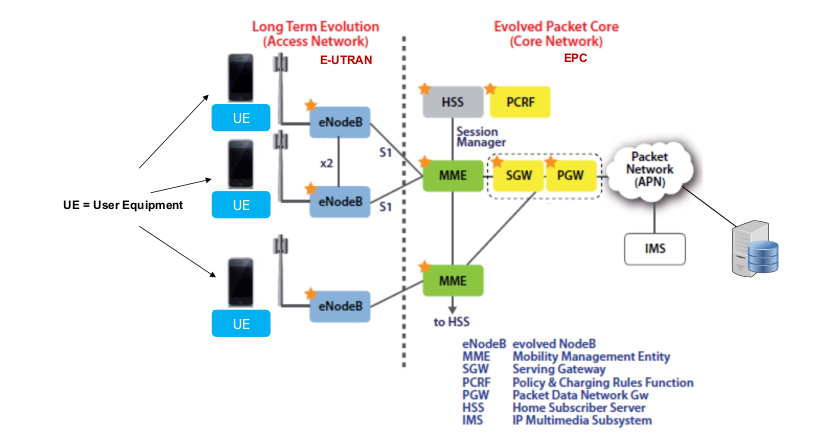
\includegraphics[width=0.6\textwidth]{architettura-lte.png}
            \caption{Architettura Lte}
            \label{fig:architettura-lte}
        \end{figure}
    \item \textbf{ECP}: l'EPC \`e stato ridefinito da zero (clean-slate), gestisce anche le risorse radio;
    \item \textbf{Bearers}: i bearer sono dei tunnel che trasportano il traffico dall'UE ad altri elementi dell'architettura, questi tunnel vengono creati per inviare il traffico attraverso alcuni nodi ritenuti i migliori per gestire il servizio dell'utente, si possono creare dei bearer per dei servizi specifici. I bearer hanno dei nomi specifici:
        \begin{itemize}
            \item radio bearer: connessione tra UE e eNodeB;
            \item s1 bearer: connessione tra eNodeB e l'S-GW (Service Gateway);
            \item s5 bearer: connette il S-GW al P-GW.
        \end{itemize}
    \item \textbf{E-UTRAN}: consistono per la maggior parte di eNodeB, la loro funzione principale \`e la gestione delle risorse, compressione degli header per migliorare le prestazioni, sicurezza, connessione all'EPC;
    \item \textbf{Control/Data Plane}: controllo: protocolli per la mobilita, sicurezza, autenticazione, dati: nuovi protocolli per per livello link e livello fisico,
\end{itemize}

In LTE c'\`e una separazione, esistono \textbf{Control/Data Plane}:
\begin{itemize}
    \item \textbf{Link Layer Protocol}: formato da:
        \begin{figure}[H]
            \centering
            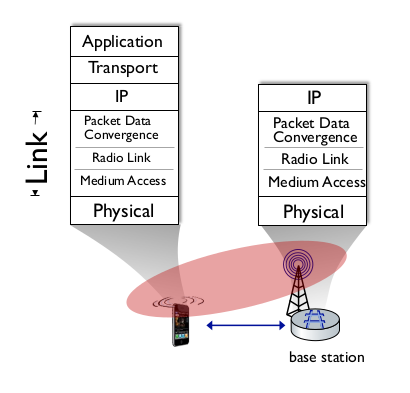
\includegraphics[width=0.6\textwidth]{link-layer.png}
            \caption{Link Layer}
            \label{fig:link-layer}
        \end{figure}
        \begin{itemize}
            \item packet data convergence: compressione e encryption;
            \item radio link control (RLC): potrebbe essere necessario frammentare i pacchetti e la ricomposizione, inoltre permette un reliable data transfer che permette una verifica dei dati, come nel wifi;
            \item medium access: richiesta di accesso, uso di slot radio;
        \end{itemize}
    \item \textbf{First Hop}: per accedere ai canali si utilizza un approccio OFDM con TDM, gli slot sono molto piccoli, grazie a questi slot piccoli gli algoritmi di assegnamento potranno asseganre pi\`u slot ad un singolo utente, tutti allocati in maniera dinamica;
    \item \textbf{Canali Fisici}: la divisione fatta da OFDM/TDM vengono detti canali, in alcuni canali vengono riservati degli slot specifici per segnali di controllo, esiste dunque un divisione tra canali di controllo e canali di dato;
    \item \textbf{Associazione di un nodo}: la BS fa un broadcast di un \textbf{primary sync signal} ogni 5ms su ogni frequenza, il terminale che riceve questo signal ne sceglio uno basandosi sulla pontenza del seganle e aspetta il \textbf{second sync signal} che contiene delle informazioni sulla BS, il primary da solo il seganle di aggancio, scelta la BS si inizia l'autenticazione e si inizializza il data plane;
    \item \textbf{Sleep Mode}: dopo 100ms di inattivit\`a il terminale entra il light sleep e viene periodicamente svegliato ogni 100ms per controllare se ci sono dei messaggi pending, se i secondi di inattivit\`a diventano 5-10s, il terminale va in deep sleep, in cui la connessione va riassociata ad una BS, se il terminale deve ricevere dei messaggi la BS pu\`o sevgliare il terminale dal deep sleep;
\end{itemize}


\section{5G}
Lo scopo \`e creare una rete wireless unificata (nuovo ordine mondiale), insieme ad altri servizi.

Per offrire tutti questi servizi bisogna disclocare i calcoli vicino all'utente (edge della rete), si ha bisogno di \textbf{network slice}, ovvero porzioni di rete dedicate ad un utente, ho bisogno di un controllore centralizzato (SDN) per assegnare le risorse.

Alcuni use cases:
\begin{itemize}
    \item eMBB (enhanced mobile brodband): definisce come in una rete si possono creare delle ditribuzioni di servizi streaming per utenti mobili;
    \item mMTC (massive machine type comunication): comunicazioni tra macchine industriali;
    \item URLLC (ultra relieable low latency comunication): comunicazioni con latenze di 1ms;
\end{itemize}

Le tecnologie usate:
\begin{itemize}
    \item forme d'onda avanzate;
    \item MIMO avanzate, con un throught maggiore di quelle di LTE;
    \item uso delle micro onde;
\end{itemize}

Core network:
\begin{itemize}
    \item SDN: controller centralizzato;
    \item NFV: funzioni virtuali eseguite;
\end{itemize}







\section{VPN (Virtual Private Network)}
Si utilizzano le VPN quando ci si vuole connettere in una rete privata passando dalla rete, per questo motivo stabilire un tipo di comuncazione va protetta. Gli elementi chiave di queste connessioni sono:
\begin{itemize}
    \item \textbf{tunnel}: incapsulamento del traffico su un canale condiviso, che in alcune situazione non potrebbe essere disponibile;
    \item \textbf{VPN gateway}: dispositivo ad-hoc per aprire e terminare dei tunnel, che dovr\`a supportare un protocollo specifico (non sempre il VPN gateway non supporta tutti i protocolli);
\end{itemize}
Il motivo per cui esistono le VPN \`e che l'alternativa sarebbe quella di posare un cavo direttamente collegato alla rete, dunque \`e comodo avere un modo di connersi ad una rete privata su una rete condivisa. Un altro motivo \`e l'utilizzo di un indirizzo IP locato in un altro paese.

In base al livello dello stack ISO/OSI \`e possibile implementare una VPN.

Gli scenari di attuazione di VPN pu\`o essere fatta in una azienda solo internamente (\textbf{Intranet VPN}) oppure pu\`o essere condivisa con pi\`u azionde o vari clienti, quindi dovranno essere presi in considerazione aspetti di sicurezza e privacy, entrando in gioco anche diversi livelli di firewall e varie autorizzazioni che vengono assegnate, si deve tenere in considerazione anche il problema dell'overlapping, ovvero avere pi\`u host con lo stesso indirizzo privato.

Quando si parla di connessione ad internet attraverso la VPN esistono due tipi di accesso:
\begin{itemize}
    \item \textbf{Centralized Internet Access}: si ha accesso alla sottorete ed a internet;
    \item \textbf{Distributed Internet Access}: solo il traffico indirizzato alla sottorete passo per la VPN, mentre il traffico verso internet passa normalmente dal default gateway;
\end{itemize}


\subsection{Deployment Model}
Con deployment model ci si focolizza sull'infrastruttura che permette di utilizzare una VPN. Le VPN devono garantire autenticazione dei peer, integrit\`a dei dati e confidenzialit\`a. Quando si fa il deploy possono essere possibili diversi tipi di tunneling.
\begin{itemize}
    \item \textbf{s2s (site 2 site) VPN tunneling}: una sottorete 1 comunica con una sottorete 2 con un tunnel;
    \item \textbf{e2e (end 2 end) VPN tunneling}: due computer in due sottoreti separate vengono connessi con un tunnel;
    \item \textbf{remote VPN tunneling}: un singolo host si collega con un border gateway delle sottorete;
\end{itemize}
Adoperare un s2s ha dei costi maggiori, infatti i due border gateway (che sono ai bordi delle sottoreti) devono gestire costi di overhead, tunnel miltipli e quelli della crittografia, mentre col e2e non si ha questo problema di gestione. Solitamente una buona soluzione implementativa \`e l'utilizzo in contemporanea di e2e e s2s.

Quando si parla di tunnel esistono diversi metodi di creazione, a differenza della soluzione si avr\`a una differenza tra performance e sicurezza, queste ultime sono inversamente proporzionali:
\begin{itemize}
    \item \textbf{Overlay Model}: nell'overlay model i tunnel vengono creati tra i due endpoint, non preccopandosi del routing.
    \item \textbf{Peer Model}: in una soluzione peer model viene creato un tunnel spezzato tra i vari router in cui si passa, quindi esisteranno tanti tunnel quanti sono i router da cui si deve passare per raggiungere la destinazione, il vantaggio di questa soluzione \`e che si pu\`o indirizzare il traffico per un percorso specifico, lo svantaggio \`e che ad ogni hop il pacchetto viene decapsulato per poi essere reincapsulato in un nuovo pacchetto quando si fa il forward.
\end{itemize}


Il tunneling in una VPN non \`e altro che l'incapsulamento di un pacchetto IP (header e payload) in un altro pacchetto IP (nel caso diVPN a livello IP), questo nouvo payload viene criptato con i protocolli GRE o IPsec.


\subsection{Livelli delle VPN}
Esisistono anche le VPNs di livello 2, vengono dette \textbf{Virtual Private LAN Service}, viene usata per emulare le funzionalit\`a delle LAN, serve anche per connettere parti della sottorete. Il tunnel viene fatto attraverso l'incapsulamento di una trama di livello 2 in pacchetto IP, per questo motivo \`e necessario avere una rete locale con una tecnologia di livello 3.

Le VPN di livello 3, hanno un routing basato su Peer o Overlay, mentre i CE possono essere connessi con e2e, s2s, remote. L'impacchettamento pu\`o essere fatto in GRE o IPsec.

Le VPN di livello 4, hanno una encapsulazione basata su TCP che ottiene un alto livello di sicurezza attraverso SSL.


\subsection{Protocolli per VPN}
Il protocollo \textbf{GRE} (Generic Routing Encapsulation) \`e uno standard per l'encapsulazione, il suo fromato \`e fatto da:
\begin{itemize}
    \item Flags: presenza di campi addizionali;
    \item s: se la destinazione non \`e raggiunta quando si \`e percorsa la lista dei router il pacchetto viene distrutto;
    \item recur: massimo numero di encapsulazioni successive;
    \item route: \`e possibile specificare un indirizzo per fare del routing, viene usato insieme al flag s;
\end{itemize}
Del protocollo GRE esiste anche una versione 1 che migliora gli acknowledge.

I protocolli di tunneling di livello sono \textbf{L2TP} (Layer 2 Tunneling Protocol), che la caratteristica di essere indipendente dal livello 2, non viene utilizzato in pratica perch\`e richiede un ulteriore encapsulamento in IPsec, ed il \textbf{PPTP} (Point To Point Tunneling) che \`e Customer provisioner, ma anche esso ha una cifratura debole oltre ad avere un sistema di chiavi proprietario.

L2TP utilizza due dispositivi per creare un tunnel, il LAC (L2TP Access Concentrator) a cui gli utenti si collegano, poi questo crea un tunnel verso il LNS (L2TP Network Server), che poi si collega alla rete locale dell'azienda.









\end{document}
